\documentclass{beamer}\usepackage[]{graphicx}\usepackage[]{color}
%% maxwidth is the original width if it is less than linewidth
%% otherwise use linewidth (to make sure the graphics do not exceed the margin)
\makeatletter
\def\maxwidth{ %
  \ifdim\Gin@nat@width>\linewidth
    \linewidth
  \else
    \Gin@nat@width
  \fi
}
\makeatother

\definecolor{fgcolor}{rgb}{0.345, 0.345, 0.345}
\newcommand{\hlnum}[1]{\textcolor[rgb]{0.686,0.059,0.569}{#1}}%
\newcommand{\hlstr}[1]{\textcolor[rgb]{0.192,0.494,0.8}{#1}}%
\newcommand{\hlcom}[1]{\textcolor[rgb]{0.678,0.584,0.686}{\textit{#1}}}%
\newcommand{\hlopt}[1]{\textcolor[rgb]{0,0,0}{#1}}%
\newcommand{\hlstd}[1]{\textcolor[rgb]{0.345,0.345,0.345}{#1}}%
\newcommand{\hlkwa}[1]{\textcolor[rgb]{0.161,0.373,0.58}{\textbf{#1}}}%
\newcommand{\hlkwb}[1]{\textcolor[rgb]{0.69,0.353,0.396}{#1}}%
\newcommand{\hlkwc}[1]{\textcolor[rgb]{0.333,0.667,0.333}{#1}}%
\newcommand{\hlkwd}[1]{\textcolor[rgb]{0.737,0.353,0.396}{\textbf{#1}}}%
\let\hlipl\hlkwb

\usepackage{framed}
\makeatletter
\newenvironment{kframe}{%
 \def\at@end@of@kframe{}%
 \ifinner\ifhmode%
  \def\at@end@of@kframe{\end{minipage}}%
  \begin{minipage}{\columnwidth}%
 \fi\fi%
 \def\FrameCommand##1{\hskip\@totalleftmargin \hskip-\fboxsep
 \colorbox{shadecolor}{##1}\hskip-\fboxsep
     % There is no \\@totalrightmargin, so:
     \hskip-\linewidth \hskip-\@totalleftmargin \hskip\columnwidth}%
 \MakeFramed {\advance\hsize-\width
   \@totalleftmargin\z@ \linewidth\hsize
   \@setminipage}}%
 {\par\unskip\endMakeFramed%
 \at@end@of@kframe}
\makeatother

\definecolor{shadecolor}{rgb}{.97, .97, .97}
\definecolor{messagecolor}{rgb}{0, 0, 0}
\definecolor{warningcolor}{rgb}{1, 0, 1}
\definecolor{errorcolor}{rgb}{1, 0, 0}
\newenvironment{knitrout}{}{} % an empty environment to be redefined in TeX

\usepackage{alltt}

% *****************************************************************************
% ADD HERE THE TOPIC OF THE LECTURE!
% \newcommand{\lecturetopic}{ALL LECTURE SLIDES}
\newcommand{\lecturetopic}{ALL SLIDES}
% *****************************************************************************



% turn off navigation symbols
\beamertemplatenavigationsymbolsempty

\title{\textbf{Data Analysis with R:} \\ \lecturetopic}
\author{Sonja Hartnack, Terence Odoch \& Muriel Buri}
\vspace{0.3cm}
\footnotesize
\institute{October 2017}
\date{ }

\setbeamertemplate{footline}[text line]{%
\parbox{\linewidth}{\vspace*{-1pt} \fontsize{3.5}{5}\selectfont Sonja Hartnack,
Terence Odoch \& Muriel Buri \hfill \lecturetopic \hfill \insertpagenumber}}

\usepackage{graphicx}
\usepackage{float}
\usepackage{animate}

\usepackage{verbatim}
\usepackage{url}
\usepackage{lmodern}
\usepackage{fancyhdr}
\usepackage{color}
\usepackage{amsmath, amssymb}
\usepackage{longtable}
\usepackage{lscape}
\usepackage{xspace}
\usepackage[normalem]{ulem}
% Use Palatino (URW Palladio) for most of the text\ldots
\usepackage[sc]{mathpazo}
% And Arial for the rest
\usepackage[scaled]{helvet}
\usepackage[latin1]{inputenc}
\usepackage{multicol} % A flexible tool to handle multicolumn documents
\usepackage{colortbl, xcolor} % enable colored rows in table
\usepackage{color} % enable colored rows in table
\usepackage{bibentry} % Include Full BibTeX Entry Inside Slides
\usepackage{nicefrac}
\usepackage{soul}

\setbeamertemplate{itemize items}[circle]

\usepackage{array}
\newcolumntype{L}[1]{>{\raggedright\let\newline\\\arraybackslash\hspace{0pt}}m{#1}}
\newcolumntype{C}[1]{>{\centering\let\newline\\\arraybackslash\hspace{0pt}}m{#1}}
\newcolumntype{R}[1]{>{\raggedleft\let\newline\\\arraybackslash\hspace{0pt}}m{#1}}

\graphicspath{{figures/}}
\usepackage[export]{adjustbox} % figure alignment
\usepackage{wrapfig} % allow for wrapfigure
\usepackage[margin=1cm]{caption}
\captionsetup{font=scriptsize, labelfont=scriptsize}

% change font family in footnote
\usepackage{footmisc}
\renewcommand*{\footnotelayout}{\tiny\sffamily}
% \renewcommand*{\footnotelayout}{\fontsize{3.5}{5}\selectfont\sffamily}

% change footer symbol
\usepackage{perpage}
\MakePerPage{footnote}
\renewcommand*{\thefootnote}{$\star$}

% change font sizes of frametitles
\setbeamerfont{frametitle}{size=\normalsize, series=\bfseries}
\setbeamerfont{framesubtitle}{size=\small, series=\bfseries}

% Settings for the references
\usepackage{natbib}
\usepackage{bibentry} % Include Full BibTeX Entry Inside Slides

% Writting the whole reference in ONE line.
% \def\newblock{\hskip .5em plus .33em minus .07em}

\setbeamerfont{title}{size=\LARGE}

\makeatletter
\def\mathcolor#1#{\@mathcolor{#1}}
\def\@mathcolor#1#2#3{%
\protect\leavevmode
\begingroup\color#1{#2}#3\endgroup
}
\makeatother

% *****************************************************************************

% {\usebackgroundtemplate{
\includegraphics[width=\paperwidth]{Printscreen_RLogo.png}}
{\usebackgroundtemplate{}}
\IfFileExists{upquote.sty}{\usepackage{upquote}}{}
\begin{document}

\bibliographystyle{plainnat}

% *****************************************************************************
% TITLE PAGE:
% *****************************************************************************

\begin{frame}[noframenumbering,plain]
\begin{columns}
\begin{column}{.3\linewidth}
\begin{center}
\includegraphics[height=.35\linewidth, width = 1.1\linewidth]{uzh_logo.pdf}
\end{center}
\end{column}
\begin{column}{0.2\linewidth}
\end{column}
\begin{column}{.3\linewidth}
\begin{center}
\includegraphics[height=.45\linewidth, width = .65\linewidth]{makere_logo.jpg}
\end{center}
\end{column}
\end{columns}
\titlepage
\end{frame}

\section{Day 1}
\usebackgroundtemplate{}
\begin{frame}
\frametitle{Goals of the course}
To be able to...
\begin{itemize}
\setlength\itemsep{1.5em}
\item import data sets to R
\item describe data with R
\item apply basic statistical tests in R
\item some ideas for more advanced statistical tools ...
\item simulate a data set similar to own research
\end{itemize}
\end{frame}

% *****************************************************************************

\begin{frame}
\frametitle{Getting to know each other}
\begin{itemize}
\setlength\itemsep{1.5em}
\item My name is ...
\item I am doing a Master / a PhD in ...
\item I hope to learn in this course how to ....
\item My personal goal for this course is ...
\end{itemize}
% REASON TO BE HERE
% (1) I love statistics and I am keen to learn more about it.
% (2) I am happy to be here are feel that I will be a bit overwhelmed.
% (3) I am here because my supervisor told me to be here.
% EXPERIENCE IN R
% (1) I have worked with R before and feel somehow familiar with it.
% (2) I have never worked with R before.
% (3) What is R?
\end{frame}

% *****************************************************************************

\begin{frame}
\frametitle{How do we reach these goals}
\begin{itemize}
\setlength\itemsep{1.2em}
\item hands on exercises with R:
\begin{itemize}
\item \texttt{chickwts}
\item \texttt{ToothGrowth}
\item \texttt{bacteria}
\item \texttt{perulung}
\item ... and others.
\end{itemize}
\item interactive discussions
\item asking a lot of questions: ask google!
\item group work
\item short motivational lectures
\end{itemize}
\end{frame}
%
% % *****************************************************************************
% %
% % Get started:
% % Short personal introduction
% % Goals
% %
% % Motivational Examples / Illustration: ChickWeight
% % Explanatory Description
% % Potential research question
%
% % A data frame in R
% % data frames: Data types (integer, numeric, factor)
%
% % Introduction to R and R Studio
% % To start with
% % Functionality R Studio and R
% %
% % Model: ANOVA
%
\begin{frame}[fragile]
\frametitle{Get started with data set: chickwts}
An experiment was conducted to measure and compare the effectiveness of various
feed supplements on the growth rate of chickens.
\begin{knitrout}\scriptsize
\definecolor{shadecolor}{rgb}{0.969, 0.969, 0.969}\color{fgcolor}\begin{kframe}
\begin{alltt}
\hlkwd{data}\hlstd{(chickwts)}
\hlkwd{head}\hlstd{(chickwts)}
\end{alltt}
\begin{verbatim}
##   weight      feed
## 1    179 horsebean
## 2    160 horsebean
## 3    136 horsebean
## 4    227 horsebean
## 5    217 horsebean
## 6    168 horsebean
\end{verbatim}
\end{kframe}
\end{knitrout}
\end{frame}
%
% *****************************************************************************

\begin{frame}[fragile]
\frametitle{Ideas for plotting the data}
\pause
\begin{knitrout}\scriptsize
\definecolor{shadecolor}{rgb}{0.969, 0.969, 0.969}\color{fgcolor}\begin{kframe}
\begin{alltt}
\hlkwd{boxplot}\hlstd{(weight} \hlopt{~} \hlstd{feed,} \hlkwc{data} \hlstd{= chickwts)}
\end{alltt}
\end{kframe}
\end{knitrout}
% EXERCISE IDEAS
% <<echo=TRUE, eval=TRUE, size="scriptsize">>=
% # hist(chickwts$weight, prob = TRUE)
% # lines(density(chickwts$weight), col = "red", lwd = 2)
% @
\end{frame}

% *****************************************************************************

\begin{frame}[fragile]
\frametitle{Ideas for analysing the data}
\pause
\begin{knitrout}\scriptsize
\definecolor{shadecolor}{rgb}{0.969, 0.969, 0.969}\color{fgcolor}\begin{kframe}
\begin{alltt}
\hlkwd{summary}\hlstd{(}\hlkwd{aov}\hlstd{(weight} \hlopt{~} \hlstd{feed,} \hlkwc{data} \hlstd{= chickwts))}
\end{alltt}
\begin{verbatim}
##             Df Sum Sq Mean Sq F value   Pr(>F)    
## feed         5 231129   46226   15.37 5.94e-10 ***
## Residuals   65 195556    3009                     
## ---
## Signif. codes:  0 '***' 0.001 '**' 0.01 '*' 0.05 '.' 0.1 ' ' 1
\end{verbatim}
\end{kframe}
\end{knitrout}
% % EXERCISE IDEAS
% <<echo=TRUE, eval=TRUE, size="scriptsize">>=
% # lm(weight ~ feed, data = chickwts)
% @
\end{frame}

% *****************************************************************************

{\usebackgroundtemplate{
\includegraphics[width=\paperwidth]{Printscreen_RLogo.png}}
\begin{frame}
\frametitle{Functionalities in R and RStudio}
\begin{itemize}
\item Source
\item Console
\item Environment, History, Files
\item Files, Plots, Packages, Help
\end{itemize}
%
\begin{center}
\includegraphics[width=0.7\paperwidth]{Printscreen_chickwts_RScreen.png}
\end{center}
%
\end{frame}

% *****************************************************************************

{\usebackgroundtemplate{
\includegraphics[width=\paperwidth]{Printscreen_RLogo.png}}
\begin{frame}[fragile]
\frametitle{Good housekeeping!}
\begin{itemize}
\setlength\itemsep{1.5em}
\item Know in which directory you are
\begin{knitrout}\scriptsize
\definecolor{shadecolor}{rgb}{0.969, 0.969, 0.969}\color{fgcolor}\begin{kframe}
\begin{alltt}
\hlkwd{getwd}\hlstd{()}
\end{alltt}
\begin{verbatim}
## [1] "/Users/murielburi/Dropbox/201710_Makerere/02_Lectures"
\end{verbatim}
\end{kframe}
\end{knitrout}
\item Set directory path
\begin{knitrout}\scriptsize
\definecolor{shadecolor}{rgb}{0.969, 0.969, 0.969}\color{fgcolor}\begin{kframe}
\begin{alltt}
\hlkwd{setwd}\hlstd{(}\hlstr{"C:\textbackslash{}\textbackslash{}Users\textbackslash{}\textbackslash{}admin\textbackslash{}\textbackslash{}201710_Makerere\textbackslash{}\textbackslash{}02_Lectures\textbackslash{}\textbackslash{}data\textbackslash{}\textbackslash{}"}\hlstd{)}
\end{alltt}
\end{kframe}
\end{knitrout}
\item Always clean up before starting with new R-Script
\begin{knitrout}\scriptsize
\definecolor{shadecolor}{rgb}{0.969, 0.969, 0.969}\color{fgcolor}\begin{kframe}
\begin{alltt}
\hlkwd{rm}\hlstd{(}\hlkwc{list}\hlstd{=}\hlkwd{ls}\hlstd{())} \hlcom{# empty workspace}
\end{alltt}
\end{kframe}
\end{knitrout}
\end{itemize}
\end{frame}

% *****************************************************************************

\begin{frame}[fragile]
\frametitle{How to get help in R}
\begin{knitrout}\scriptsize
\definecolor{shadecolor}{rgb}{0.969, 0.969, 0.969}\color{fgcolor}\begin{kframe}
\begin{alltt}
\hlopt{?}\hlstd{chickwts}
\end{alltt}
\end{kframe}
\end{knitrout}
Also, have a look at the examples at the end of the help pages.
\end{frame}

% *****************************************************************************

\begin{frame}
\frametitle{Exercise 1}
\end{frame}


% *****************************************************************************

\begin{frame}
\frametitle{A data frame in R: \texttt{chickwts}}
\begin{center}
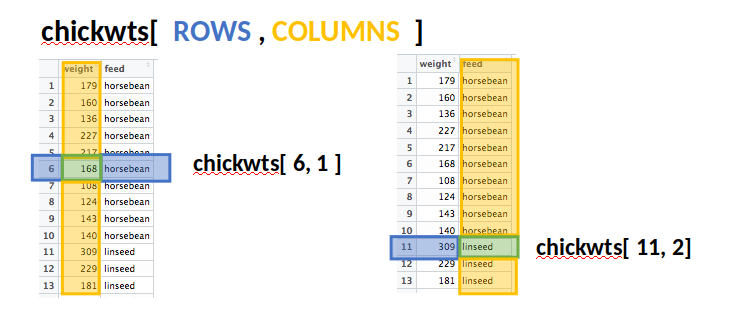
\includegraphics[width = \linewidth]{Printscreen_Data_Frame_in_R.png}
\end{center}
\end{frame}

% *****************************************************************************

\begin{frame}[fragile]
\frametitle{Rows and columns of a data frame: \texttt{chickwts}}
Values of ...
\begin{knitrout}\scriptsize
\definecolor{shadecolor}{rgb}{0.969, 0.969, 0.969}\color{fgcolor}\begin{kframe}
\begin{alltt}
\hlcom{# ... all columns of sixth observation:}
\hlstd{chickwts[}\hlnum{6}\hlstd{, ]}

\hlcom{# ... all columns of sixth to eleventh observation:}
\hlstd{chickwts[}\hlnum{6}\hlopt{:}\hlnum{11}\hlstd{, ]}

\hlcom{# ... all columns of sixth, eleventh and twentieth observation:}
\hlstd{chickwts[}\hlkwd{c}\hlstd{(}\hlnum{6}\hlstd{,} \hlnum{11}\hlstd{,} \hlnum{20}\hlstd{), ]}

\hlcom{# ... all rows of first column (weight):}
\hlstd{chickwts[ ,} \hlnum{1}\hlstd{]}

\hlcom{# ... all rows of second column (feed):}
\hlstd{chickwts[ ,} \hlnum{2}\hlstd{]}
\hlcom{# or use the "$" sign as a reference to column "feed":}
\hlstd{chickwts}\hlopt{$}\hlstd{feed}
\end{alltt}
\end{kframe}
\end{knitrout}
\end{frame}

% *****************************************************************************

\begin{frame}[fragile]
\frametitle{What is a data frame in R?}
A data frame is used for storing a list of vectors of equal length.
For example, the following variable df is a data frame containing three vectors n, s, b.
\begin{knitrout}\scriptsize
\definecolor{shadecolor}{rgb}{0.969, 0.969, 0.969}\color{fgcolor}\begin{kframe}
\begin{alltt}
\hlstd{n} \hlkwb{<-} \hlkwd{c}\hlstd{(}\hlnum{2}\hlstd{,} \hlnum{3}\hlstd{,} \hlnum{5}\hlstd{)}
\hlstd{s} \hlkwb{<-} \hlkwd{c}\hlstd{(}\hlstr{"aa"}\hlstd{,} \hlstr{"bb"}\hlstd{,} \hlstr{"cc"}\hlstd{)}
\hlstd{b} \hlkwb{<-} \hlkwd{c}\hlstd{(}\hlnum{TRUE}\hlstd{,} \hlnum{FALSE}\hlstd{,} \hlnum{TRUE}\hlstd{)}
\hlstd{df} \hlkwb{<-} \hlkwd{data.frame}\hlstd{(n, s, b)} \hlcom{# df is a data frame}
\end{alltt}
\end{kframe}
\end{knitrout}
Following are the characteristics of a data frame:
\begin{itemize}
\item The column names should be non-empty.
\item The row names should be unique.
\item The data stored in a data frame can be of numeric, factor or character type.
\item Each column should contain same number of data items.
\end{itemize}
\end{frame}

% *****************************************************************************

\begin{frame}[fragile]
\frametitle{Data frame in R}
\begin{knitrout}\scriptsize
\definecolor{shadecolor}{rgb}{0.969, 0.969, 0.969}\color{fgcolor}\begin{kframe}
\begin{alltt}
\hlstd{a} \hlkwb{<-} \hlkwd{c}\hlstd{(}\hlnum{1}\hlstd{,} \hlnum{2}\hlstd{,} \hlnum{3}\hlstd{,} \hlnum{4}\hlstd{)}
\hlstd{a}
\end{alltt}
\begin{verbatim}
## [1] 1 2 3 4
\end{verbatim}
\begin{alltt}
\hlkwd{data.frame}\hlstd{(a)}
\end{alltt}
\begin{verbatim}
##   a
## 1 1
## 2 2
## 3 3
## 4 4
\end{verbatim}
\begin{alltt}
\hlstd{b} \hlkwb{<-} \hlkwd{c}\hlstd{(}\hlstr{"d"}\hlstd{,} \hlstr{"h"}\hlstd{,} \hlstr{"h"}\hlstd{,} \hlstr{"d"}\hlstd{)}
\hlstd{dat} \hlkwb{<-} \hlkwd{data.frame}\hlstd{(a, b)}
\hlstd{dat}
\end{alltt}
\begin{verbatim}
##   a b
## 1 1 d
## 2 2 h
## 3 3 h
## 4 4 d
\end{verbatim}
\end{kframe}
\end{knitrout}
\end{frame}

% *****************************************************************************

\begin{frame}[fragile]
\frametitle{Data frame in R: How to add a vector variable}
\begin{knitrout}\scriptsize
\definecolor{shadecolor}{rgb}{0.969, 0.969, 0.969}\color{fgcolor}\begin{kframe}
\begin{alltt}
\hlstd{c} \hlkwb{<-} \hlkwd{factor}\hlstd{(}\hlkwd{c}\hlstd{(}\hlstr{"male"}\hlstd{,} \hlstr{"female"}\hlstd{,} \hlstr{"male"}\hlstd{,} \hlstr{"female"}\hlstd{),}
                \hlkwc{levels} \hlstd{=} \hlkwd{c}\hlstd{(}\hlstr{"female"}\hlstd{,} \hlstr{"male"}\hlstd{))}
\hlstd{dat}\hlopt{$}\hlstd{c} \hlkwb{<-} \hlstd{c} \hlcom{# use "$" to refer to the additional vector variable}
\hlstd{dat}
\end{alltt}
\begin{verbatim}
##   a b      c
## 1 1 d   male
## 2 2 h female
## 3 3 h   male
## 4 4 d female
\end{verbatim}
\begin{alltt}
\hlcom{# What is the dimension (number of rows and columns) of our data frame?}
\hlkwd{dim}\hlstd{(dat)} \hlcom{# 4 rows and 3 columns}
\end{alltt}
\begin{verbatim}
## [1] 4 3
\end{verbatim}
\end{kframe}
\end{knitrout}
\end{frame}

% *****************************************************************************

\begin{frame}
\frametitle{Exercise 2}
\end{frame}

% *****************************************************************************

\begin{frame}[fragile]
\frametitle{How to install a package}
\begin{knitrout}\scriptsize
\definecolor{shadecolor}{rgb}{0.969, 0.969, 0.969}\color{fgcolor}\begin{kframe}
\begin{alltt}
\hlkwd{install.packages}\hlstd{(}\hlstr{"MASS"}\hlstd{)}
\hlkwd{library}\hlstd{(}\hlstr{"MASS"}\hlstd{)}
\hlkwd{data}\hlstd{(bacteria)}
\hlopt{?}\hlstd{bacteria}
\end{alltt}
\end{kframe}
\end{knitrout}
\end{frame}

% *****************************************************************************

\begin{frame}[fragile]
\frametitle{How to install a package}
\begin{center}
\includegraphics[width = \linewidth]{Printscreen_Rscreen.png}
\end{center}
\end{frame}

% *****************************************************************************

\begin{frame}[fragile]
\frametitle{Exercise 3}
\end{frame}

% *****************************************************************************
\section{Day 2}
\usebackgroundtemplate{}
\begin{frame}[fragile]
\frametitle{How to google for getting help in R}
\begin{itemize}
\setlength\itemsep{1.5em}
\item Google for \textbf{select observations in R}.
\end{itemize}
\end{frame}

% *****************************************************************************

{\usebackgroundtemplate{
\includegraphics[width=\paperwidth]{Printscreen_RLogo.png}}
\begin{frame}[fragile]
\frametitle{Creating and assigning objects in R}
Objects are assigned values using $<-$ , an arrow formed out of $<$ and $-$.
For example, the following command assigns the value 1 to the object \texttt{a}.
\begin{knitrout}\scriptsize
\definecolor{shadecolor}{rgb}{0.969, 0.969, 0.969}\color{fgcolor}\begin{kframe}
\begin{alltt}
\hlstd{a} \hlkwb{<-} \hlnum{1} \hlcom{# ALWAYS use "gets" assignment operator!}
\hlcom{# a = 1 # DO NOT USE the equal sign as the assignment operator!}
\end{alltt}
\end{kframe}
\end{knitrout}
After this assignment, the object \texttt{a} contains the value 1.
Another assignment to the same object will change the content.
\begin{knitrout}\scriptsize
\definecolor{shadecolor}{rgb}{0.969, 0.969, 0.969}\color{fgcolor}\begin{kframe}
\begin{alltt}
\hlstd{a} \hlkwb{<-} \hlnum{5}
\end{alltt}
\end{kframe}
\end{knitrout}
\end{frame}

% *****************************************************************************

\begin{frame}[fragile]
\frametitle{Examples of assigned objects: Single number}
\begin{knitrout}\scriptsize
\definecolor{shadecolor}{rgb}{0.969, 0.969, 0.969}\color{fgcolor}\begin{kframe}
\begin{alltt}
\hlstd{a} \hlkwb{<-} \hlnum{1}
\hlstd{b} \hlkwb{<-} \hlnum{2}
\hlstd{c} \hlkwb{<-} \hlstd{a} \hlopt{+} \hlstd{b} \hlcom{# c = 3}
\hlstd{c}
\end{alltt}
\begin{verbatim}
## [1] 3
\end{verbatim}
\end{kframe}
\end{knitrout}
\end{frame}

% *****************************************************************************

\begin{frame}[fragile]
\frametitle{Examples of assigned objects: Vector}
\begin{knitrout}\scriptsize
\definecolor{shadecolor}{rgb}{0.969, 0.969, 0.969}\color{fgcolor}\begin{kframe}
\begin{alltt}
\hlstd{a} \hlkwb{<-} \hlkwd{c}\hlstd{(}\hlnum{1}\hlstd{,} \hlnum{2}\hlstd{,} \hlnum{3}\hlstd{,} \hlnum{4}\hlstd{,} \hlnum{5}\hlstd{)}
\hlstd{b} \hlkwb{<-} \hlnum{1}
\hlstd{c} \hlkwb{<-} \hlstd{a} \hlopt{+} \hlstd{b}
\hlstd{c}
\end{alltt}
\begin{verbatim}
## [1] 2 3 4 5 6
\end{verbatim}
\end{kframe}
\end{knitrout}
\end{frame}

% *****************************************************************************

\begin{frame}[fragile]
\frametitle{Examples of assigned objects: Model}
\begin{knitrout}\scriptsize
\definecolor{shadecolor}{rgb}{0.969, 0.969, 0.969}\color{fgcolor}\begin{kframe}
\begin{alltt}
\hlstd{anova_model} \hlkwb{<-} \hlkwd{aov}\hlstd{(weight} \hlopt{~} \hlstd{feed,} \hlkwc{data} \hlstd{= chickwts)}
\hlkwd{summary}\hlstd{(anova_model)}
\end{alltt}
\begin{verbatim}
##             Df Sum Sq Mean Sq F value   Pr(>F)    
## feed         5 231129   46226   15.37 5.94e-10 ***
## Residuals   65 195556    3009                     
## ---
## Signif. codes:  0 '***' 0.001 '**' 0.01 '*' 0.05 '.' 0.1 ' ' 1
\end{verbatim}
\end{kframe}
\end{knitrout}
\end{frame}

% *****************************************************************************

\begin{frame}[fragile]
\frametitle{Examples of assigned objects: Dataframe}

\begin{knitrout}\scriptsize
\definecolor{shadecolor}{rgb}{0.969, 0.969, 0.969}\color{fgcolor}\begin{kframe}
\begin{alltt}
\hlstd{bac} \hlkwb{<-} \hlstd{bacteria}
\hlkwd{str}\hlstd{(bac)} \hlcom{# $ week: int  0 2 4 11 0 2 6 11 0 2 ...}
\end{alltt}
\begin{verbatim}
## 'data.frame':	220 obs. of  6 variables:
##  $ y   : Factor w/ 2 levels "n","y": 2 2 2 2 2 2 1 2 2 2 ...
##  $ ap  : Factor w/ 2 levels "a","p": 2 2 2 2 1 1 1 1 1 1 ...
##  $ hilo: Factor w/ 2 levels "hi","lo": 1 1 1 1 1 1 1 1 2 2 ...
##  $ week: int  0 2 4 11 0 2 6 11 0 2 ...
##  $ ID  : Factor w/ 50 levels "X01","X02","X03",..: 1 1 1 1 2 2 2 2 3 3 ...
##  $ trt : Factor w/ 3 levels "placebo","drug",..: 1 1 1 1 3 3 3 3 2 2 ...
\end{verbatim}
\begin{alltt}
\hlstd{bac_sub} \hlkwb{<-} \hlkwd{subset}\hlstd{(bac, week} \hlopt{==} \hlnum{2}\hlstd{)}
\hlkwd{str}\hlstd{(bac_sub)} \hlcom{# $ week: int  2 2 2 2 2 2 2 2 2 2 ...}
\end{alltt}
\begin{verbatim}
## 'data.frame':	44 obs. of  6 variables:
##  $ y   : Factor w/ 2 levels "n","y": 2 2 2 2 2 2 1 2 2 2 ...
##  $ ap  : Factor w/ 2 levels "a","p": 2 1 1 2 2 1 1 2 2 2 ...
##  $ hilo: Factor w/ 2 levels "hi","lo": 1 1 2 2 2 2 1 1 2 1 ...
##  $ week: int  2 2 2 2 2 2 2 2 2 2 ...
##  $ ID  : Factor w/ 50 levels "X01","X02","X03",..: 1 2 3 4 5 6 7 8 9 11 ...
##  $ trt : Factor w/ 3 levels "placebo","drug",..: 1 3 2 1 1 2 3 1 1 1 ...
\end{verbatim}
\end{kframe}
\end{knitrout}
\end{frame}

% *****************************************************************************

\begin{frame}[fragile]
\frametitle{Structure of a R objects}
The \texttt{str} function displays the \texttt{str}ucture of an R object. One line for each "basic" structure is displayed.
\begin{knitrout}\scriptsize
\definecolor{shadecolor}{rgb}{0.969, 0.969, 0.969}\color{fgcolor}\begin{kframe}
\begin{verbatim}
## 'data.frame':	44 obs. of  6 variables:
##  $ y   : Factor w/ 2 levels "n","y": 2 2 2 2 2 2 1 2 2 2 ...
##  $ ap  : Factor w/ 2 levels "a","p": 2 1 1 2 2 1 1 2 2 2 ...
##  $ hilo: Factor w/ 2 levels "hi","lo": 1 1 2 2 2 2 1 1 2 1 ...
##  $ week: int  2 2 2 2 2 2 2 2 2 2 ...
##  $ ID  : Factor w/ 50 levels "X01","X02","X03",..: 1 2 3 4 5 6 7 8 9 11 ...
##  $ trt : Factor w/ 3 levels "placebo","drug",..: 1 3 2 1 1 2 3 1 1 1 ...
\end{verbatim}
\end{kframe}
\end{knitrout}
\end{frame}

% *****************************************************************************

\begin{frame}[fragile]
\frametitle{Exercise 4}
\end{frame}

% *****************************************************************************

\begin{frame}[fragile]
\frametitle{Data types in R}
\begin{itemize}
\item numeric
\begin{knitrout}\scriptsize
\definecolor{shadecolor}{rgb}{0.969, 0.969, 0.969}\color{fgcolor}\begin{kframe}
\begin{alltt}
\hlkwd{data}\hlstd{(ToothGrowth)}
\hlstd{ToothGrowth}\hlopt{$}\hlstd{len[}\hlnum{1}\hlopt{:}\hlnum{6}\hlstd{]}
\end{alltt}
\begin{verbatim}
## [1]  4.2 11.5  7.3  5.8  6.4 10.0
\end{verbatim}
\begin{alltt}
\hlkwd{class}\hlstd{(ToothGrowth}\hlopt{$}\hlstd{len[}\hlnum{1}\hlopt{:}\hlnum{6}\hlstd{])}
\end{alltt}
\begin{verbatim}
## [1] "numeric"
\end{verbatim}
\end{kframe}
\end{knitrout}
\item integers
\begin{knitrout}\scriptsize
\definecolor{shadecolor}{rgb}{0.969, 0.969, 0.969}\color{fgcolor}\begin{kframe}
\begin{alltt}
\hlstd{bacteria}\hlopt{$}\hlstd{week[}\hlnum{1}\hlopt{:}\hlnum{6}\hlstd{]}
\end{alltt}
\begin{verbatim}
## [1]  0  2  4 11  0  2
\end{verbatim}
\begin{alltt}
\hlkwd{class}\hlstd{(bacteria}\hlopt{$}\hlstd{week[}\hlnum{1}\hlopt{:}\hlnum{6}\hlstd{])}
\end{alltt}
\begin{verbatim}
## [1] "integer"
\end{verbatim}
\end{kframe}
\end{knitrout}
\item (un/ordered) factor
\begin{knitrout}\scriptsize
\definecolor{shadecolor}{rgb}{0.969, 0.969, 0.969}\color{fgcolor}\begin{kframe}
\begin{alltt}
\hlstd{chickwts}\hlopt{$}\hlstd{feed[}\hlnum{1}\hlopt{:}\hlnum{6}\hlstd{]}
\end{alltt}
\begin{verbatim}
## [1] horsebean horsebean horsebean horsebean horsebean horsebean
## Levels: casein horsebean linseed meatmeal soybean sunflower
\end{verbatim}
\begin{alltt}
\hlkwd{levels}\hlstd{(chickwts}\hlopt{$}\hlstd{feed)[}\hlnum{1}\hlopt{:}\hlnum{3}\hlstd{]}
\end{alltt}
\begin{verbatim}
## [1] "casein"    "horsebean" "linseed"
\end{verbatim}
\end{kframe}
\end{knitrout}
\end{itemize}
\end{frame}

% *****************************************************************************

\begin{frame}[fragile]
\frametitle{Data types in R: Ordered Factors}
Ordinal variables are represented as ordered factors:
\begin{knitrout}\scriptsize
\definecolor{shadecolor}{rgb}{0.969, 0.969, 0.969}\color{fgcolor}\begin{kframe}
\begin{alltt}
\hlstd{bac_growth} \hlkwb{<-} \hlkwd{c}\hlstd{(}\hlstr{"none"}\hlstd{,} \hlstr{"+"}\hlstd{,} \hlstr{"++"}\hlstd{,} \hlstr{"+"}\hlstd{,} \hlstr{"+++"}\hlstd{,} \hlstr{"+"}\hlstd{,} \hlstr{"none"}\hlstd{)} \hlcom{# vector}
\hlstd{bac_growth} \hlkwb{<-} \hlkwd{factor}\hlstd{(bac_growth,} \hlkwc{levels} \hlstd{=} \hlkwd{c}\hlstd{(}\hlstr{"none"}\hlstd{,} \hlstr{"+"}\hlstd{,} \hlstr{"++"}\hlstd{,} \hlstr{"+++"}\hlstd{),}
               \hlkwc{order} \hlstd{=} \hlnum{TRUE}\hlstd{)}
\hlstd{bac_growth}
\end{alltt}
\begin{verbatim}
## [1] none +    ++   +    +++  +    none
## Levels: none < + < ++ < +++
\end{verbatim}
\begin{alltt}
\hlcom{#}
\hlstd{mood} \hlkwb{<-} \hlkwd{c}\hlstd{(}\hlstr{"OK"}\hlstd{,} \hlstr{"Well"}\hlstd{,} \hlstr{"Super"}\hlstd{,} \hlstr{"Super"}\hlstd{,} \hlstr{"Don't ask"}\hlstd{,} \hlstr{"OK"}\hlstd{)} \hlcom{# vector}
\hlstd{mood} \hlkwb{<-} \hlkwd{factor}\hlstd{(mood,} \hlkwc{levels} \hlstd{=} \hlkwd{c}\hlstd{(}\hlstr{"Don't ask"}\hlstd{,} \hlstr{"Well"}\hlstd{,} \hlstr{"OK"}\hlstd{,} \hlstr{"Super"}\hlstd{),}
               \hlkwc{order} \hlstd{=} \hlnum{TRUE}\hlstd{)}
\hlstd{mood}
\end{alltt}
\begin{verbatim}
## [1] OK        Well      Super     Super     Don't ask OK       
## Levels: Don't ask < Well < OK < Super
\end{verbatim}
\end{kframe}
\end{knitrout}
\end{frame}

% *****************************************************************************

\begin{frame}[fragile]
\frametitle{Exercise 5}
\end{frame}

% *****************************************************************************

\begin{frame}[fragile]
\frametitle{Exercise 6}
\end{frame}

% *****************************************************************************

\begin{frame}[fragile]
\frametitle{Rules for importing data into R (from Excel)}
\begin{itemize}
\item First row of excel sheet contains \textbf{variable names}: \newline
\texttt{y, ap, hilo, week, ID, trt}.
\item Columns of excel sheet represent \textbf{variables}.
\item Rows of excel sheet represent \textbf{observations per individual}
(except for the first row).
\end{itemize}
\begin{center}
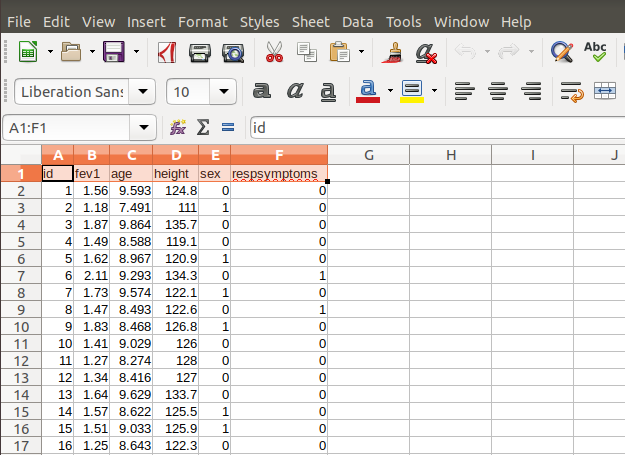
\includegraphics[width = \linewidth]{Printscreen_ExcelSheet.png}
\end{center}
\end{frame}

% *****************************************************************************

\begin{frame}[fragile]
\frametitle{Rules for naming variables}
Variable names should ..
\begin{itemize}
\item start with a letter (not a number): \texttt{y, ap, hilo, week, ID, trt}
\item longer variables names should be separated with dots: \texttt{time.in.weeks}
\item do not use special characters, such as /, \#, $@$, \&, $\star$, ...
\end{itemize}
\end{frame}

% *****************************************************************************

\begin{frame}[fragile]
\frametitle{How to import Excel files into R?}
\framesubtitle{Three major steps: Excel file preparation}
\begin{center}
\includegraphics[width = \linewidth]{Printscreen_Import_Data_to_R_1.png}
\end{center}
\end{frame}

% *****************************************************************************

\begin{frame}[fragile]
\frametitle{How to import Excel files into R?}
\framesubtitle{Three major steps: Excel file preparation}
\begin{center}
\includegraphics[width = \linewidth]{Printscreen_Import_Data_to_R_2.png}
\end{center}
\end{frame}

% *****************************************************************************

\begin{frame}[fragile]
\frametitle{How to import Excel files into R?}
\framesubtitle{Three major steps: Save raw data file as .csv}
\begin{center}
\includegraphics[width = \linewidth]{Printscreen_Import_Data_to_R_3.png}
\end{center}
\end{frame}

% *****************************************************************************

\begin{frame}[fragile]
\frametitle{How to import Excel files into R?}
\framesubtitle{Three major steps: Import data into R}
\end{frame}

% *****************************************************************************

\begin{frame}[fragile]
\frametitle{How to import Excel files into R?}
\framesubtitle{Three major steps: Import data into R}
\begin{center}
\includegraphics[width = \linewidth]{Printscreen_Import_Data_to_R_4.png}
\end{center}
\end{frame}

% *****************************************************************************

\begin{frame}[fragile]
\frametitle{How to import Excel files into R?}
\framesubtitle{Three major steps: Import data into R}
\begin{center}
\includegraphics[width = \linewidth]{Printscreen_Import_Data_to_R_5.png}
\end{center}
\end{frame}


% *****************************************************************************

\begin{frame}[fragile]
\frametitle{How to import Excel files into R?}
\begin{knitrout}\scriptsize
\definecolor{shadecolor}{rgb}{0.969, 0.969, 0.969}\color{fgcolor}\begin{kframe}
\begin{alltt}
\hlcom{# Import .csv file with the help of the read.csv function}
\hlcom{# Be sure to add sep = ";" so that we separate the columns.}
\hlstd{lung} \hlkwb{<-} \hlkwd{read.csv}\hlstd{(}\hlstr{"C:\textbackslash{}\textbackslash{}Users\textbackslash{}\textbackslash{}Exercises\textbackslash{}\textbackslash{}data\textbackslash{}\textbackslash{}perulung_ems.csv"}\hlstd{,} \hlkwc{sep} \hlstd{=} \hlstr{";"}\hlstd{)}
\hlkwd{head}\hlstd{(lung)}
\hlkwd{str}\hlstd{(lung)}
\end{alltt}
\end{kframe}
\end{knitrout}

\end{frame}

% *****************************************************************************

\begin{frame}[fragile]
\frametitle{Exercise 7: perulung}
Data from a study of lung function among children living in a deprived suburb of
Lima, Peru. Data taken from Kirkwood and Sterne, 2nd edition. \newline
Variables:
\begin{itemize}
\item \texttt{fev1}:  in liter, ''forced expiratory volume in 1 second'' measured
by a spirometer. This is the maximum volume of air which the children could breath
out in 1 second
\item \texttt{age}: in years
\item \texttt{height}: in cm
\item \texttt{sex}: 0 = girl, 1 = boy
\item \texttt{respsymp}: respiratory symptoms experienced by the child over the
previous 12 months
\end{itemize}
\end{frame}

% *****************************************************************************
\section{Day 3}
\usebackgroundtemplate{}
\begin{frame}{Why do we need Statistics?}
\Large{\textbf{Repeatability of results:}} \newline
\textbf{Statistical science} allows us to
estimate what might happen if an experiment was repeated - but without having to
actually repeat it!
\end{frame}

% *****************************************************************************

\begin{frame}{Why do we need Statistics?}
\vspace{0.5cm}
\begin{itemize}
\setlength\itemsep{1.5em}
\item Study results must be shown to be robust, i.e. real and not due to random
chance
\item Best way to demonstrate this is to repeat the same experiment/study many
times each with {\bfseries different} subjects (animals) drawn from the {\bfseries
same study population} and show that the result is truly repeatable
\item It is generally totally impractical, in terms of both time and resources,
to repeat an experiment many times!
\end{itemize}
\vspace{0.5cm}
\end{frame}

% *****************************************************************************

\begin{frame}
\frametitle{Why do we need Statistics?}
\begin{itemize}
\setlength\itemsep{1.5em}
\item Instead of repeating the experiment many times {\bfseries probability
theory i.e. statistics} is used to {\bfseries estimate} what might have happened
if the experiment had been repeated
\item A mathematical model is used to fill this ``data gap''
\item Generally the most difficult task in statistics is to decide what ``model''
is most appropriate for a given experiment
\end{itemize}
\vspace{0.5cm}
\end{frame}

% *****************************************************************************

\begin{frame}
\frametitle{What is Statistics? - A definition}
A set of analytical tools designed to quantify uncertainty
\vspace{0.3cm}
\begin{itemize}
\setlength\itemsep{1.5em}
\item If an experiment or procedure is repeated, how likely is it that the new
results will be similar to those already observed?
\item What is the likely variation in results if the experiment was repeated?
\end{itemize}\vspace{0.5cm}
\end{frame}

% *****************************************************************************

\begin{frame}
\frametitle{What is Statistics? - A definition}
The key scientific purpose of statistics
\vspace{0.5cm}
\begin{itemize}
\setlength\itemsep{1.5em}
\item to provide {\bfseries evidence} of the existence of some ``effect'' of
scientific interest
\item i.e. evidence based medicine
\end{itemize}
\vspace{0.5cm}
\end{frame}

% *****************************************************************************

\begin{frame}
\frametitle{As a reminder: The importance of study design}
Even the most sophisticated statistical analyses cannot rescue a poorly
designed study
\begin{itemize}
\setlength\itemsep{1.5em}
\item[$\rightarrow$] unreliable results
\item[$\rightarrow$] inability to answer the main research question
\end{itemize}
\vspace{0.5cm}
\end{frame}

% *****************************************************************************

\begin{frame}
\frametitle{Putting Statistics in Context}
\begin{itemize}
\setlength\itemsep{1.5em}
\item The vast majority of analyses can be done in a straightforward fashion -
just remember and always use common sense as a guide - be skeptical!
\item It is very easy to get ``lost'' in the statistical software and technical
jargon, which differs markedly between different software packages. Terminology
can also differ greatly between textbooks...
\item Wikipedia is as good a resource as any for finding out about different
statistical tests and terminology
\end{itemize}
\end{frame}

% *****************************************************************************

\begin{frame}
\frametitle{Exploratory Data Analysis}
\begin{itemize}
\item It is crucially important to explore your data fully before considering any
``formal'' statistical analyses\pause
\item What explorations are done depends on the objective of the study - the
research question(s)\pause
\item Helps to decide what kind of formal statistical analyses might be most
appropriate for the data available\pause
\item What a simple descriptive analysis {\bfseries does not} provide is evidence
of whether the observed treatment effects are large enough to be notable once
sampling variation has been accounted - that is the role of formal analyses,
e.g. hypothesis testing
\end{itemize}
\end{frame}

% *****************************************************************************

\begin{frame}[plain]
\begin{figure}
\includegraphics[scale=0.45]{samplingfig1.pdf}
\end{figure}
\end{frame}

% *****************************************************************************

\begin{frame}
\frametitle{Continuous (Integers / Numeric) Data Summaries}
 \begin{itemize}
\item {\tt Mean} - a measure of location. Always examine the average value of
the response variable(s) for the different ``treatment'' effects in your data
\item {\tt Median} - a robust single value summary of a set of data (50\% quantile
point) - most useful in highly skewed data or data with outliers
\item {\tt Standard deviation (sd)} - a measure of spread, how variable the data
are
\item {\tt Standard error of the mean (se)} - an estimate of how far the sample
mean is likely to be from the population mean
\item and others:  {\tt min, max, range, IQR, ...}
\end{itemize}
\end{frame}

% *****************************************************************************

\usebackgroundtemplate{
\includegraphics[width=\paperwidth]{Printscreen_RLogo.png}}
% \usebackgroundtemplate{}
\begin{frame}[fragile]
\frametitle{Continuous (Integers / Numeric) Data Summaries}
\begin{knitrout}
\definecolor{shadecolor}{rgb}{0.969, 0.969, 0.969}\color{fgcolor}\begin{kframe}
\begin{alltt}
\hlkwd{mean}\hlstd{(x)} \hlcom{# mean}

\hlkwd{median}\hlstd{(x)} \hlcom{# median}

\hlkwd{sd}\hlstd{(x)} \hlcom{# standard deviation}

\hlkwd{min}\hlstd{(x)} \hlcom{# minimum}

\hlkwd{max}\hlstd{(x)} \hlcom{# maximum}

\hlkwd{range}\hlstd{(x)} \hlcom{# range}

\hlkwd{IQR}\hlstd{(x)} \hlcom{# interquartile range}
\end{alltt}
\end{kframe}
\end{knitrout}
\end{frame}

% *****************************************************************************

% \usebackgroundtemplate{
\includegraphics[width=\paperwidth]{Printscreen_RLogo.png}}
\usebackgroundtemplate{}
\begin{frame}[plain]
\frametitle{Continuous Data Summaries}
\begin{figure}
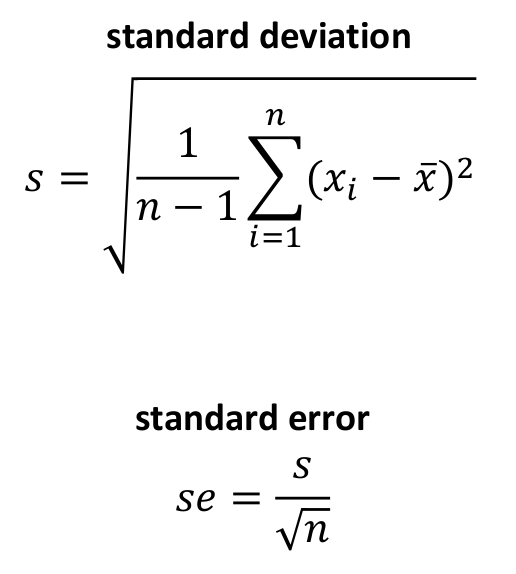
\includegraphics[scale=0.45]{se_sd.pdf}
\end{figure}
\end{frame}

% *****************************************************************************

\begin{frame}
\frametitle{Continuous Data Summaries}
\framesubtitle{Combination of continuous and continuous}
\begin{itemize}
\item {\tt Correlation coefficient} - a measure association between two continuous variables (common but somewhat limited)\\\vspace{0.3cm}
\includegraphics[scale=0.3]{correlation0.pdf}
\end{itemize}
\end{frame}

% *****************************************************************************

\begin{frame}[plain]
\frametitle{Correlation coefficient}
\framesubtitle{Combination of continuous and continuous}
\begin{figure}
\includegraphics[scale=0.45]{correlation1.pdf}
\end{figure}
\end{frame}

% *****************************************************************************

\usebackgroundtemplate{
\includegraphics[width=\paperwidth]{Printscreen_RLogo.png}}
% \usebackgroundtemplate{}
\begin{frame}[fragile]
\frametitle{Correlation coefficient}
\framesubtitle{Combination of continuous with continuous / ordinal}
\begin{knitrout}
\definecolor{shadecolor}{rgb}{0.969, 0.969, 0.969}\color{fgcolor}\begin{kframe}
\begin{alltt}
\hlcom{# Test for Association/Correlation Between}
\hlcom{# Paired Samples}
\hlkwd{cor.test}\hlstd{(data}\hlopt{$}\hlstd{x, data}\hlopt{$}\hlstd{y,} \hlkwc{method} \hlstd{=} \hlstr{"pearson"}\hlstd{)}
\hlkwd{cor.test}\hlstd{(data}\hlopt{$}\hlstd{x, data}\hlopt{$}\hlstd{y,} \hlkwc{method} \hlstd{=} \hlstr{"spearman"}\hlstd{)}

\hlcom{# Scatterplot(s)}
\hlkwd{pairs}\hlstd{(data}\hlopt{$}\hlstd{x} \hlopt{~} \hlstd{data}\hlopt{$}\hlstd{y)}
\hlkwd{pairs}\hlstd{(data)}
\end{alltt}
\end{kframe}
\end{knitrout}
\end{frame}

% *****************************************************************************

\begin{frame}[fragile]
\frametitle{Correlation coefficient}
\framesubtitle{Combination of continuous with factors}
\begin{knitrout}
\definecolor{shadecolor}{rgb}{0.969, 0.969, 0.969}\color{fgcolor}\begin{kframe}
\begin{alltt}
\hlkwd{tapply}\hlstd{(data}\hlopt{$}\hlstd{x.cont, data}\hlopt{$}\hlstd{y.fac, mean)}

\hlkwd{tapply}\hlstd{(data}\hlopt{$}\hlstd{x.cont, data}\hlopt{$}\hlstd{y.fac, median)}

\hlkwd{tapply}\hlstd{(data}\hlopt{$}\hlstd{x.cont, data}\hlopt{$}\hlstd{y.fac, sd)}
\end{alltt}
\end{kframe}
\end{knitrout}
\end{frame}

% *****************************************************************************

\begin{frame}[fragile]
\frametitle{Ordinal Data Summaries}
\begin{itemize}
\setlength\itemsep{1.3em}
\item {\tt Median} - a robust single value summary of a set of data
(50\% quantile point) - most useful in highly skewed data or data with outliers
\item {\tt e.g.10th and 90th percentile} - a measure of spread, how variable
the data are
\begin{knitrout}
\definecolor{shadecolor}{rgb}{0.969, 0.969, 0.969}\color{fgcolor}\begin{kframe}
\begin{alltt}
\hlkwd{quantile}\hlstd{(x,} \hlkwc{probs} \hlstd{=} \hlkwd{c}\hlstd{(}\hlnum{0.1}\hlstd{,} \hlnum{0.9}\hlstd{))}
\end{alltt}
\end{kframe}
\end{knitrout}
\item {\tt proportions} - e.g. percentage per grade
\begin{knitrout}
\definecolor{shadecolor}{rgb}{0.969, 0.969, 0.969}\color{fgcolor}\begin{kframe}
\begin{alltt}
\hlkwd{prop.table}\hlstd{(}\hlkwd{table}\hlstd{(data}\hlopt{$}\hlstd{x.fac))}
\hlkwd{prop.table}\hlstd{(}\hlkwd{table}\hlstd{(data}\hlopt{$}\hlstd{x.fac, data}\hlopt{$}\hlstd{y.fac))}
\end{alltt}
\end{kframe}
\end{knitrout}
\end{itemize}
\end{frame}

% *****************************************************************************

\begin{frame}[fragile]
\frametitle{Nominal Data Summaries}
\begin{itemize}
\item {\tt proportions} - percentage within the different categories
\item {\tt contingency tables} e. g. 2x2
\begin{knitrout}
\definecolor{shadecolor}{rgb}{0.969, 0.969, 0.969}\color{fgcolor}\begin{kframe}
\begin{alltt}
\hlkwd{table}\hlstd{(data}\hlopt{$}\hlstd{x.fac)}
\hlkwd{table}\hlstd{(data}\hlopt{$}\hlstd{x.fac, data}\hlopt{$}\hlstd{y.fac)}
\hlkwd{prop.table}\hlstd{(}\hlkwd{table}\hlstd{(data}\hlopt{$}\hlstd{x.fac))}
\hlkwd{prop.table}\hlstd{(}\hlkwd{table}\hlstd{(data}\hlopt{$}\hlstd{x.fac, data}\hlopt{$}\hlstd{y.fac))}
\end{alltt}
\end{kframe}
\end{knitrout}
\end{itemize}
\end{frame}

% *****************************************************************************

\begin{frame}
\frametitle{Exercise 8}
\end{frame}

% *****************************************************************************

% \usebackgroundtemplate{
\includegraphics[width=\paperwidth]{Printscreen_RLogo.png}}
\usebackgroundtemplate{}
\begin{frame}[fragile]
\frametitle{How to deal with missing values in R? (1/3)}
\begin{itemize}
\setlength\itemsep{1.3em}
\item In R, missing values are represented by the symbol \textbf{NA}
(not available).
\item Impossible values (e. g., dividing by zero) are represented by the symbol
\textbf{NaN} (not a number).
\item Ask yourself why a \textbf{NA} and / or \textbf{NaN} occurs!
\end{itemize}
\end{frame}

% *****************************************************************************

% \usebackgroundtemplate{
\includegraphics[width=\paperwidth]{Printscreen_RLogo.png}}
\usebackgroundtemplate{}
\begin{frame}[fragile]
\frametitle{How to deal with missing values in R? (2/3)}
\begin{itemize}
\setlength\itemsep{1.3em}
\item Testing for Missing Values
\begin{knitrout}\scriptsize
\definecolor{shadecolor}{rgb}{0.969, 0.969, 0.969}\color{fgcolor}\begin{kframe}
\begin{alltt}
\hlstd{vec1} \hlkwb{<-} \hlkwd{c}\hlstd{(}\hlnum{1}\hlstd{,} \hlnum{2}\hlstd{,} \hlnum{3}\hlstd{,} \hlnum{NA}\hlstd{)}
\hlkwd{is.na}\hlstd{(vec1)} \hlcom{# returns a vector (FALSE, FALSE, FALSE, TRUE)}
\hlcom{# The TRUE indicates the position of the NA in vec1.}
\end{alltt}
\end{kframe}
\end{knitrout}
\item Recoding Values to Missing
\begin{knitrout}\scriptsize
\definecolor{shadecolor}{rgb}{0.969, 0.969, 0.969}\color{fgcolor}\begin{kframe}
\begin{alltt}
\hlcom{# recode specific values (e. g. 0.001) to missing for variable x}
\hlcom{# select rows where x is 0.001 and recode value in column x with NA}
\hlstd{dat}\hlopt{$}\hlstd{x[dat}\hlopt{$}\hlstd{x} \hlopt{==} \hlnum{0.001}\hlstd{]} \hlkwb{<-} \hlnum{NA}
\end{alltt}
\end{kframe}
\end{knitrout}
\end{itemize}
\end{frame}

% *****************************************************************************

\begin{frame}[fragile]
\frametitle{How to deal with missing values in R? (3/3)}
\begin{itemize}
\setlength\itemsep{1.3em}
\item Excluding Missing Values from specific function calls
\begin{knitrout}\scriptsize
\definecolor{shadecolor}{rgb}{0.969, 0.969, 0.969}\color{fgcolor}\begin{kframe}
\begin{alltt}
\hlstd{a} \hlkwb{<-} \hlkwd{c}\hlstd{(}\hlnum{1}\hlstd{,} \hlnum{2}\hlstd{,} \hlnum{NA}\hlstd{,} \hlnum{3}\hlstd{)}
\hlkwd{mean}\hlstd{(a)} \hlcom{# returns NA}
\hlkwd{mean}\hlstd{(a,} \hlkwc{na.rm}\hlstd{=}\hlnum{TRUE}\hlstd{)} \hlcom{# returns 2}
\end{alltt}
\end{kframe}
\end{knitrout}
\item Check for complete cases with function \texttt{complete.cases(...)}
\begin{knitrout}\scriptsize
\definecolor{shadecolor}{rgb}{0.969, 0.969, 0.969}\color{fgcolor}\begin{kframe}
\begin{alltt}
\hlcom{# list rows of data that have missing values}
\hlstd{dat[}\hlopt{!}\hlkwd{complete.cases}\hlstd{(dat),]}
\hlstd{subdat} \hlkwb{<-} \hlstd{dat[}\hlkwd{complete.cases}\hlstd{(dat),]}
\end{alltt}
\end{kframe}
\end{knitrout}
\item Create new dataset without missing data with function \texttt{na.omit(...)}
\begin{knitrout}\scriptsize
\definecolor{shadecolor}{rgb}{0.969, 0.969, 0.969}\color{fgcolor}\begin{kframe}
\begin{alltt}
\hlstd{new.dat} \hlkwb{<-} \hlkwd{na.omit}\hlstd{(dat)}
\end{alltt}
\end{kframe}
\end{knitrout}
\end{itemize}
\end{frame}

% *****************************************************************************

% \usebackgroundtemplate{
\includegraphics[width=\paperwidth]{Printscreen_RLogo.png}}
\usebackgroundtemplate{}
\begin{frame}[fragile]
\frametitle{How to check your data for plausibility?}
\begin{itemize}
\setlength\itemsep{1.3em}
\item Ask yourself what can go wrong?
\item Implausible values?
\item Impossible values?
\item Logical errors?
\end{itemize}
\end{frame}

% *****************************************************************************

\usebackgroundtemplate{
\includegraphics[width=\paperwidth]{Printscreen_RLogo.png}}
% \usebackgroundtemplate{}
\begin{frame}[fragile]
\frametitle{Exercise 9A: Plausibility Checks}
\end{frame}

% *****************************************************************************

\begin{frame}[fragile]
\frametitle{Exercise 9B: Missing Values}
\end{frame}

% *****************************************************************************

\begin{frame}[fragile]
\frametitle{Exercise 10}
\end{frame}

% *****************************************************************************
\section{Day 4}
% \usebackgroundtemplate{
\includegraphics[width=\paperwidth]{Printscreen_RLogo.png}}
\usebackgroundtemplate{}
\begin{frame}
\frametitle{Basic Statistical Tests}
Study data is collected for a purpose - to answer one or more specific
scientific questions. The classical way to perform a formal statistical
analyses of these data is to formulate these research questions into
statistical {\bfseries hypothesis tests}. \\
\vspace{0.5cm}
In this section we will go through a simple example in detail to highlight
some of the important concepts - the general approach for more complex
analyses is exactly same. \emph{Note: the precise technical details are
much less important than the concepts!}
\end{frame}

% *****************************************************************************

\begin{frame}
\frametitle{Simple Example - One Population}
{\bfseries After six weeks will the mean weight of a chicken be more than 250
grams?}\\
There are 71 observations in \texttt{chickwts} from which to answer this
question. This can be formulated into a statistical hypothesis test. A
hypothesis test has two parts, the null hypothesis and the alternative
hypothesis. This is typically written as follows:
\begin{eqnarray}
H_0:\quad \mu &\le& 250 \nonumber\\
H_A:\quad \mu &>& 250 \nonumber
\end{eqnarray}
where $\mu$ is the mean weight in the {\bfseries population} of
chickens from which the sample of 71 chickens was drawn. Remember - we know the
mean weight in the sample of chickens is greater than 250 it is the
{\bfseries population} of chickens which we are interested in.
\end{frame}

% *****************************************************************************

\begin{frame}
\frametitle{Simple Example - One Population}
{\bfseries After six weeks will the mean weight of a chicken be at least 250 grams?}
\begin{eqnarray}
H_0:\quad \mu &\le& 250 \nonumber\\
H_A:\quad \mu &>& 250 \nonumber
\end{eqnarray}
The null hypothesis ($H_0$) is the default situation, sometimes called the
``state of nature''. In a treatment-control trial, $H_0$ is typically that
the effect of the treatment is not different from the control. In this
example our default position is that the mean weight of chickens is
{\bfseries $\le{250}$}. This is called a single-sided hypothesis test.
\end{frame}

% *****************************************************************************

\usebackgroundtemplate{
\includegraphics[width=\paperwidth]{Printscreen_RLogo.png}}
% \usebackgroundtemplate{}
\begin{frame}[fragile]
\frametitle{Simple Example - One Population}
We now analyse the 71 observations to see whether there is evidence to
{\bfseries REJECT} the null hypothesis $H_0$, and if the null hypothesis is
rejected then we can conclude that the available evidence supports the
alternative hypothesis.
\begin{knitrout}
\definecolor{shadecolor}{rgb}{0.969, 0.969, 0.969}\color{fgcolor}\begin{kframe}
\begin{alltt}
\hlkwd{t.test}\hlstd{(chickwts}\hlopt{$}\hlstd{weight,} \hlkwc{mu} \hlstd{=} \hlnum{250}\hlstd{)}
\end{alltt}
\end{kframe}
\end{knitrout}
Note that hypothesis testing is concerned with finding evidence in support
of the null hypothesis $H_0$ - the default situation -  rather than evidence
in favour of the alternative hypothesis.
\end{frame}

% *****************************************************************************

% \usebackgroundtemplate{
\includegraphics[width=\paperwidth]{Printscreen_RLogo.png}}
\usebackgroundtemplate{}
\begin{frame}
\frametitle{One Sample t-test}
For the chicken weights data an appropriate formal analyses is to use a
{\bfseries one-sample t-test}, why this test is appropriate will be discussed
later. This analysis involves calculating a simple summary statistic - called
a $t$-statistic - which we do entirely from the observed data.
\begin{equation}
T_{obs}=\frac{\bar{x}-\mu}{s/\sqrt{n}} \nonumber
\end{equation}
where $\bar{x}$ is the sample mean, $s$ the sample standard deviation and $\mu$
is the population mean in the null hypothesis which we wish to test for. We then
look up the value of $T_{obs}$ in a set of statistical tables/computer to see
what the answer is to our research question.
\end{frame}

% *****************************************************************************

\begin{frame}
\frametitle{Important concept - sampling }
\begin{center}
Why is $T_{obs}=\frac{\bar{x}-\mu}{s/\sqrt(n)}$ called a $t$-statistic?
\end{center}
\vspace{0.2cm}
If another sample of 71 chickens from the same population were weighed then the
values for $\bar{x}$ and $s$ would be different, and hence the value for $T_{obs}$.
If this was repeated many times and a histogram/Q-Q/P-P plot produced of the
values for $T_{obs}$ then this would follow the shape of a known distribution
- {\bfseries student-$t$ probability distribution}. It is this piece of
mathematics - knowing what the sampling distribution of $T_{obs}$ is -
which allows us to infer information about the population of chickens from
which our original 71 chickens were sampled - without actually having to
collect lots and lots of other samples of chickens! Mathematical theory is
used to fill this data gap.
\end{frame}

% *****************************************************************************

\begin{frame}
\frametitle{\texttt{chickwts}: t-test}
\begin{equation}
T_{obs}=\frac{261.31-250}{78.07/\sqrt{71}}=1.22 \nonumber
\end{equation}
Put the values for the sample mean and standard deviation into the t-statistic
formula along with the $\mu=250$. We now look up the value of this in a
t-distribution reference table. All this calculation will be done for you in
R but it is important to understand the general process as this is the same
for hypothesis testing in other more complex analyses.
\end{frame}

% *****************************************************************************

\begin{frame}\frametitle{One Sample, one-sided, t-test}
\includegraphics[angle=270,scale=0.35]{fig1.pdf}
\end{frame}

% *****************************************************************************

\begin{frame}
\frametitle{Important concept - $p$-values}
\begin{itemize}
\item The result of a hypothesis test is usually communicated in the form of a
{\bfseries $p$-value}
\item The interpretation of a $p$-value is of crucial importance - it is the
\emph{probability that the test statistic takes values at least as extreme
as that observed {\bfseries assuming that $H_0$ is true}}
\item Exactly what {\bfseries at least as extreme as} refers to depends on
the alternative hypothesis $H_A$.
\item This may sound rather abstract but it is usually obvious in practice
\end{itemize}
\end{frame}

% *****************************************************************************

\begin{frame}
\frametitle{Simple Example - One Population}
 {\bfseries After six weeks will the mean weight of a chicken be at least 250 grams?}
\begin{eqnarray}
H_0:\quad \mu &\le& 250 \nonumber\\
H_A:\quad \mu &>& 250 \nonumber
\end{eqnarray}
The alternative hypothesis is $\mu > 250$ so in this test
{\bfseries at least as extreme as} in the definition of a $p$-value is the
probability of observing a t-statistic which is $>1.22$
{\bfseries assuming that $H_0$ is true} - this is why 250 was used for $\mu$ when calculating $T_{obs}$.
\\\vspace{0.2cm}
\end{frame}

% *****************************************************************************

\begin{frame}\frametitle{One Sample, one-sided, t-test}
\includegraphics[angle=270,scale=0.35]{fig2.pdf}
\end{frame}

% *****************************************************************************

\begin{frame}
\frametitle{Research Question}
The purpose of this hypothesis test analysis is to answer a very specific
scientific question:
\begin{center}{\bfseries After six weeks will the mean weight of a chicken be
more than 250 grams?}\end{center}
So what is our answer?\\\vspace{0.3cm}
The $p$-value for this hypothesis test is 0.113. Based on this value we can either
{\bfseries \large reject} $H_0$ and conclude that the mean weight of chickens
in the population is likely to be greater than 250 grams or else we can
{\bfseries \large accept} $H_0$ where the mean chicken weight is less than 250 grams.
\\\vspace{0.3cm}
\end{frame}

% *****************************************************************************

\begin{frame}
\frametitle{Research Question - be pragmatic with $p$-values}
\vspace{0.2cm}
By convention a $p$-value of less than 0.05 is considered to provide reasonable
evidence for rejecting $H_0$. A $p$-value of between 0.05 and 0.1 might be
considered as weak evidence against $H_0$. Values of less that 0.01 are generally
considered as very strong evidence for rejecting $H_0$. It is {\bfseries always}
best to provide a $p$-value in any analyses to let the reviewer/client see the
strength of evidence rather than simply claiming statistically significant
findings!
\vspace{0.2cm}
\end{frame}

% *****************************************************************************

\begin{frame}
\frametitle{Communicating Results of Hypothesis Tests}
Transparency is essential - the devil can be in the detail - which at the very
least should comprise:
\begin{itemize}
\item[i.] what hypothesis was being tested - be clear and precise
\item[ii.] what statistical test was used
\item[iii.] what the $p$-value is
\item[iv.] what the treatment effect is (more later).
\end{itemize}
\vspace{0.2cm}
This is particularly crucial if the analyses are to be given to someone
\emph{else} to then make a judgment on the scientific significance.
\end{frame}

% *****************************************************************************

\begin{frame}
\frametitle{Two-sided Tests: One Population}
{\bfseries After six weeks will the mean weight of a chicken {\bfseries be equal}
to 250 grams?}\\
This is now a two sided hypothesis test:
\begin{eqnarray}
H_0:\quad \mu &=& 250 \nonumber \\
H_A:\quad \mu &\ne& 250 \nonumber
\end{eqnarray}
This time the hypothesis test is asking how much evidence is there in our sample
data to conclude that in the population of all chickens the mean weight is not
equal to 250 grams.
\end{frame}

% *****************************************************************************

\usebackgroundtemplate{
\includegraphics[width=\paperwidth]{Printscreen_RLogo.png}}
% \usebackgroundtemplate{}
\begin{frame}[fragile]
\frametitle{Two-sided Tests: One Population}


\begin{knitrout}
\definecolor{shadecolor}{rgb}{0.969, 0.969, 0.969}\color{fgcolor}\begin{kframe}
\begin{alltt}
\hlkwd{t.test}\hlstd{(chickwts}\hlopt{$}\hlstd{weight,} \hlkwc{mu} \hlstd{=} \hlnum{250}\hlstd{)}
\end{alltt}
\begin{verbatim}
## 
## 	One Sample t-test
## 
## data:  chickwts$weight
## t = 1.2206, df = 70, p-value = 0.2263
## alternative hypothesis: true mean is not equal to 250
## 95 percent confidence interval:
##  242.8301 279.7896
## sample estimates:
## mean of x 
##  261.3099
\end{verbatim}
\end{kframe}
\end{knitrout}
\end{frame}

% *****************************************************************************

% \usebackgroundtemplate{
\includegraphics[width=\paperwidth]{Printscreen_RLogo.png}}
\usebackgroundtemplate{}
\begin{frame}
\frametitle{Two-sided Tests}
\vspace{0.2cm}
A two-sided test is similar to a one-sided test - the key difference is in what
is now defined as {\bfseries at least as extreme} in the definition of the $p$-value.
This time the alternative hypothesis refers to observing a value of
{\bfseries either} $\bar{x}>250$ or $\bar{x}< -250$ {\bfseries assuming that $H_0$ is true},
which using the t-test approach is equivalent to the probability of observing
$T_{obs}>1.22$ or $T_{obs}<-1.22$ which we can again look up in reference tables.
\vspace{0.2cm}
\end{frame}

% *****************************************************************************

\begin{frame}
\frametitle{One Sample, two-sided, t-test}
\includegraphics[angle=270,scale=0.35]{fig3}
\end{frame}

% *****************************************************************************

\begin{frame}
\frametitle{Two-sided Tests}
\begin{itemize}
\item The two-sided t-test has a $p$-value which is exactly double the single
sided test
\item Think! - intuitively the $p$-value should be less for a single sided test
as the research question you are asking is much narrower e.g. greater than
250 grams, as opposed to whether the mean chicken weight might be {\bfseries either}
less than 250 grams {\bfseries or greater} than 250 grams.\\
\vspace{0.2cm}
$\rightarrow$ You are using the same amount of information (71 observations)
to answer a narrower research question and so all else being equal you should
expect a ``more powerful'' analyses (e.g. a lower $p$-value all else being equal)
\end{itemize}
\end{frame}

% *****************************************************************************

\usebackgroundtemplate{
\includegraphics[width=\paperwidth]{Printscreen_RLogo.png}}
% \usebackgroundtemplate{}
\begin{frame}
\frametitle{Exercise 11}
\end{frame}

% *****************************************************************************

% \usebackgroundtemplate{
\includegraphics[width=\paperwidth]{Printscreen_RLogo.png}}
\usebackgroundtemplate{}
\begin{frame}
\frametitle{Chisquare-Test}
\begin{center}
\includegraphics[width=0.7\paperwidth]{chi_square_test.png}
\end{center}
\end{frame}

% *****************************************************************************

% \usebackgroundtemplate{
\includegraphics[width=\paperwidth]{Printscreen_RLogo.png}}
\usebackgroundtemplate{}
\begin{frame}
\frametitle{The Chisquare Distribution}
\begin{center}
\includegraphics[width=0.7\paperwidth]{chi_square_distr.png}
\end{center}
\end{frame}

% *****************************************************************************

% \usebackgroundtemplate{
\includegraphics[width=\paperwidth]{Printscreen_RLogo.png}}
\usebackgroundtemplate{}
\begin{frame}
\frametitle{Exact Fisher Test: Permutation Test}
\begin{center}
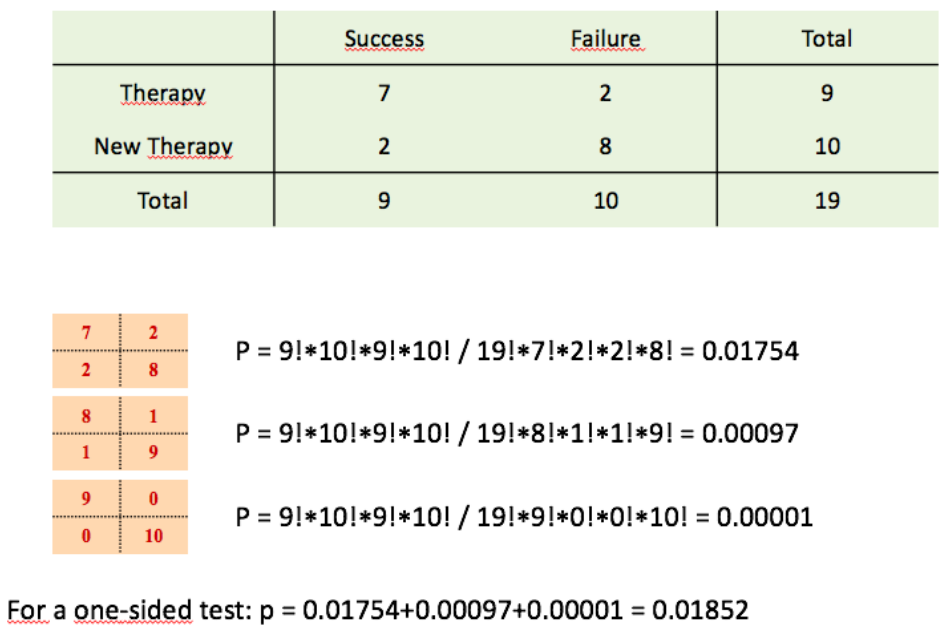
\includegraphics[width=0.7\paperwidth]{fisher_test.png}
\end{center}
\end{frame}

% *****************************************************************************

\usebackgroundtemplate{
\includegraphics[width=\paperwidth]{Printscreen_RLogo.png}}
% \usebackgroundtemplate{}
\begin{frame}
\frametitle{Exercise 12}
\end{frame}

% *****************************************************************************

\usebackgroundtemplate{
\includegraphics[width=\paperwidth]{Printscreen_RLogo.png}}
% \usebackgroundtemplate{}
\begin{frame}[fragile]
\frametitle{Plotting in R}
\pause
\begin{itemize}
\setlength\itemsep{1.5em}
\item Continuous data
\begin{itemize}
\item Histogram
\item Boxplot
\end{itemize}
\item Nominal / Ordinal data
\begin{itemize}
\item Barplot
\item Mosaicplot
\item Scatterplots
\end{itemize}
\end{itemize}
\end{frame}

% *****************************************************************************

\usebackgroundtemplate{
\includegraphics[width=\paperwidth]{Printscreen_RLogo.png}}
% \usebackgroundtemplate{}
\begin{frame}
\frametitle{Exercise 13A and 13B}
\end{frame}

\usebackgroundtemplate{
\includegraphics[width=\paperwidth]{Printscreen_RLogo.png}}
% \usebackgroundtemplate{}
\begin{frame}
\frametitle{Exercise 14}
\end{frame}

% *****************************************************************************
\section{Day 5}
% \usebackgroundtemplate{
\includegraphics[width=\paperwidth]{Printscreen_RLogo.png}}
\usebackgroundtemplate{}
\begin{frame}
\frametitle{Overview: ANOVA and linear models}
\begin{itemize}
\item Introduction to ANOVA
\item How to run an ANOVA in R
\item Checking model assumptions in R
\item Multiple comparisons options in R
\item ANOVA as a special case of a linear model
\item The simple linear regression model
\item The multiple linear regression model
\item Model selection: $R^2$ and AIC
\item Two-way Interactions in R (Day 6)
\item Confounding (Day 6)

\end{itemize}
\end{frame}

% *****************************************************************************

% \usebackgroundtemplate{
\includegraphics[width=\paperwidth]{Printscreen_RLogo.png}}
\usebackgroundtemplate{}
\begin{frame}
\frametitle{Hypothesis Testing - One Way ANOVA}
We have seen how to perform hypothesis tests when comparing two populations using
the two sample t-test. In many analyses we may have multiple populations - for
example suppose we have a treatment which has a number of different levels
high/medium/low/placebo, or equivalently a number of different treatments.
What then is the hypothesis we wish to test?\\
\vspace{0.3cm} {\bfseries Is there a difference in the effect of the treatment?}
\begin{eqnarray}
H_0&:&\quad \mu_1=\mu_2=\dots=\mu_k\nonumber\\
H_A&:&\quad \mbox{at least one pair of }\mu_1,\dots,\mu_k \quad \text{are different}
\nonumber
\end{eqnarray}
where $\mu_1,\dots,\mu_k$ denote the mean effect of treatment levels 1 through $k$.
\end{frame}

% *****************************************************************************

% \usebackgroundtemplate{
\includegraphics[width=\paperwidth]{Printscreen_RLogo.png}}
\usebackgroundtemplate{}
\begin{frame}
\frametitle{One Way ANOVA}
Analysis of variance, {\bfseries ANOVA}, to analyze differences between group
means. The observed variance in the outcome variable is partitioned into
components attributable to different sources of variation.
\end{frame}

% *****************************************************************************

% \usebackgroundtemplate{
\includegraphics[width=\paperwidth]{Printscreen_RLogo.png}}
\usebackgroundtemplate{}
\begin{frame}
\frametitle{ANOVA  estimates three sample variances (sum of squares)}
\begin{itemize}
\item a total variance based on all observation deviations from the grand mean
\item a variance based on the group mean deviations from the grand mean
\item an (error) variance based on all the observation deviations from their
group mean
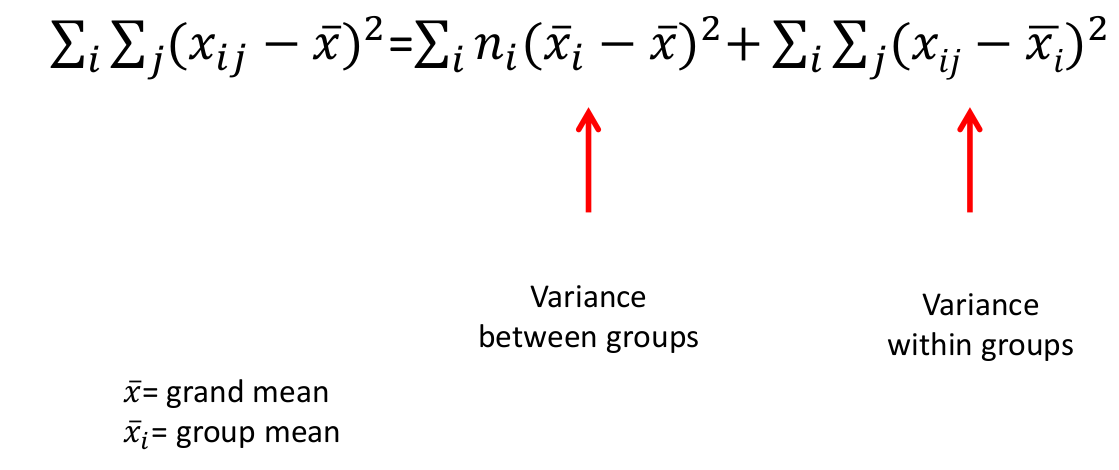
\includegraphics[scale=0.4]{anova.pdf}
\end{itemize}
\end{frame}

% *****************************************************************************

% \usebackgroundtemplate{\includegraphics[width=\paperwidth]{Printscreen_RLogo.png}}
\usebackgroundtemplate{}
\begin{frame}
\frametitle{F-test / F-distribution}
An {\bfseries F-test}, a statistical test, in which the test statistic has an
F-distribution under the null hypothesis is used to assess statistical significance
in an ANOVA.
\begin{itemize}
\item degrees of freedom
\includegraphics[scale=0.4]{F}
\end{itemize}
\end{frame}

% *****************************************************************************

\usebackgroundtemplate{\includegraphics[width=\paperwidth]{Printscreen_RLogo.png}}
% \usebackgroundtemplate{}
\begin{frame}[fragile]
\frametitle{ANOVA in R with \texttt{chickwts}}
\begin{knitrout}
\definecolor{shadecolor}{rgb}{0.969, 0.969, 0.969}\color{fgcolor}\begin{kframe}
\begin{alltt}
\hlkwd{data}\hlstd{(chickwts)}
\hlkwd{boxplot}\hlstd{(chickwts}\hlopt{$}\hlstd{weight} \hlopt{~} \hlstd{chickwts}\hlopt{$}\hlstd{feed)}
\end{alltt}
\end{kframe}

{\centering \includegraphics[width=0.7\linewidth]{figure/unnamed-chunk-41-1} 

}



\end{knitrout}
\end{frame}

% *****************************************************************************

\usebackgroundtemplate{\includegraphics[width=\paperwidth]{Printscreen_RLogo.png}}
% \usebackgroundtemplate{}
\begin{frame}[fragile]
\frametitle{ANOVA in R with \texttt{chickwts}}
\begin{knitrout}\scriptsize
\definecolor{shadecolor}{rgb}{0.969, 0.969, 0.969}\color{fgcolor}\begin{kframe}
\begin{alltt}
\hlcom{# aov.mod <- aov(chickwts$weight ~ chickwts$feed)}
\hlstd{aov.mod} \hlkwb{<-} \hlkwd{aov}\hlstd{(weight} \hlopt{~} \hlstd{feed,} \hlkwc{data} \hlstd{= chickwts)}
\hlcom{# What objects can we extract from a anova model?}
\hlkwd{objects}\hlstd{(aov.mod)}
\end{alltt}
\begin{verbatim}
##  [1] "assign"        "call"          "coefficients"  "contrasts"    
##  [5] "df.residual"   "effects"       "fitted.values" "model"        
##  [9] "qr"            "rank"          "residuals"     "terms"        
## [13] "xlevels"
\end{verbatim}
\begin{alltt}
\hlcom{#}
\hlkwd{summary}\hlstd{(aov.mod)}
\end{alltt}
\begin{verbatim}
##             Df Sum Sq Mean Sq F value   Pr(>F)    
## feed         5 231129   46226   15.37 5.94e-10 ***
## Residuals   65 195556    3009                     
## ---
## Signif. codes:  0 '***' 0.001 '**' 0.01 '*' 0.05 '.' 0.1 ' ' 1
\end{verbatim}
\end{kframe}
\end{knitrout}
\end{frame}

% *****************************************************************************

% \usebackgroundtemplate{\includegraphics[width=\paperwidth]{Printscreen_RLogo.png}}
\usebackgroundtemplate{}
\begin{frame}
\frametitle{Overview: Checking model assumptions}
\begin{itemize}
\setlength\itemsep{1.2em}
\item mean(residuals) = 0
\item Residuals are normally distributed (qqnorm, qqplot)
\item Variance homoscedasticity (Bartlett \& Levene's Test)
\item Cook's distance: Influential data points
\item Any pattern(s)?
\end{itemize}
\end{frame}

% *****************************************************************************

\usebackgroundtemplate{\includegraphics[width=\paperwidth]{Printscreen_RLogo.png}}
% \usebackgroundtemplate{}
\begin{frame}[fragile]
\frametitle{Checking model residuals: mean(residuals) = 0}
''Unexplained rest of the model''
\begin{knitrout}\scriptsize
\definecolor{shadecolor}{rgb}{0.969, 0.969, 0.969}\color{fgcolor}\begin{kframe}
\begin{alltt}
\hlcom{# What are residuals?}
\hlstd{chickwts}\hlopt{$}\hlstd{residuals} \hlkwb{<-} \hlkwd{residuals}\hlstd{(aov.mod)}
\hlkwd{tapply}\hlstd{(chickwts}\hlopt{$}\hlstd{weight, chickwts}\hlopt{$}\hlstd{feed, mean)}
\end{alltt}
\begin{verbatim}
##    casein horsebean   linseed  meatmeal   soybean sunflower 
##  323.5833  160.2000  218.7500  276.9091  246.4286  328.9167
\end{verbatim}
\begin{alltt}
\hlstd{chickwts[}\hlkwd{c}\hlstd{(}\hlnum{1}\hlopt{:}\hlnum{3}\hlstd{),]}
\end{alltt}
\begin{verbatim}
##   weight      feed residuals
## 1    179 horsebean      18.8
## 2    160 horsebean      -0.2
## 3    136 horsebean     -24.2
\end{verbatim}
\begin{alltt}
\hlcom{# Save residuals to an objects and check mean of residuals}
\hlstd{aov.mod.resid} \hlkwb{<-} \hlkwd{residuals}\hlstd{(aov.mod)}
\hlkwd{mean}\hlstd{(aov.mod.resid)}
\end{alltt}
\begin{verbatim}
## [1] 7.573045e-16
\end{verbatim}
\end{kframe}
\end{knitrout}
\end{frame}

% *****************************************************************************

\usebackgroundtemplate{\includegraphics[width=\paperwidth]{Printscreen_RLogo.png}}
% \usebackgroundtemplate{}
\begin{frame}[fragile]
\frametitle{Checking model residuals: Residuals normally distributed}
''Unexplained rest of the model''
\begin{knitrout}\scriptsize
\definecolor{shadecolor}{rgb}{0.969, 0.969, 0.969}\color{fgcolor}\begin{kframe}
\begin{alltt}
\hlkwd{par}\hlstd{(}\hlkwc{mfrow}\hlstd{=}\hlkwd{c}\hlstd{(}\hlnum{1}\hlstd{,}\hlnum{1}\hlstd{))}
\hlkwd{qqnorm}\hlstd{(aov.mod.resid)}
\hlkwd{qqline}\hlstd{(aov.mod.resid,} \hlkwc{col} \hlstd{=} \hlstr{"red"}\hlstd{,} \hlkwc{lwd} \hlstd{=} \hlnum{3}\hlstd{,} \hlkwc{lty} \hlstd{=} \hlnum{2}\hlstd{)}
\end{alltt}
\end{kframe}

{\centering \includegraphics[width=0.3\linewidth]{figure/unnamed-chunk-44-1} 

}


\begin{kframe}\begin{alltt}
\hlcom{# Shapiro-Wilk test (dependent on sample size --> limited use)}
\hlkwd{shapiro.test}\hlstd{(aov.mod.resid)}
\end{alltt}
\begin{verbatim}
## 
## 	Shapiro-Wilk normality test
## 
## data:  aov.mod.resid
## W = 0.98616, p-value = 0.6272
\end{verbatim}
\end{kframe}
\end{knitrout}
\end{frame}

% *****************************************************************************

\usebackgroundtemplate{\includegraphics[width=\paperwidth]{Printscreen_RLogo.png}}
% \usebackgroundtemplate{}
\begin{frame}[fragile]
\frametitle{Checking model residuals: Variance homoscedasticity (1/3)}
\framesubtitle{Hypothesis tests}
\begin{knitrout}\scriptsize
\definecolor{shadecolor}{rgb}{0.969, 0.969, 0.969}\color{fgcolor}\begin{kframe}
\begin{alltt}
\hlcom{# Bartlett Test}
\hlkwd{bartlett.test}\hlstd{(chickwts}\hlopt{$}\hlstd{weight} \hlopt{~} \hlstd{chickwts}\hlopt{$}\hlstd{feed)}
\end{alltt}
\begin{verbatim}
## 
## 	Bartlett test of homogeneity of variances
## 
## data:  chickwts$weight by chickwts$feed
## Bartlett's K-squared = 3.2597, df = 5, p-value = 0.66
\end{verbatim}
\begin{alltt}
\hlcom{# Levene's Test}
\hlcom{# library("Rcmdr")}
\hlcom{# levene.test(chickwts$weight ~ chickwts$feed)}
\end{alltt}
\end{kframe}
\end{knitrout}
\end{frame}

% *****************************************************************************

\usebackgroundtemplate{\includegraphics[width=\paperwidth]{Printscreen_RLogo.png}}
% \usebackgroundtemplate{}
\begin{frame}[fragile]
\frametitle{Checking model residuals: Variance homoscedasticity (2/3)}
\framesubtitle{Graphical interpretation is better!}
\begin{knitrout}\scriptsize
\definecolor{shadecolor}{rgb}{0.969, 0.969, 0.969}\color{fgcolor}\begin{kframe}
\begin{alltt}
\hlcom{# Plot fitted against residual values}
\hlkwd{plot}\hlstd{(}\hlkwd{fitted.values}\hlstd{(aov.mod),} \hlkwd{residuals}\hlstd{(aov.mod))}
\end{alltt}
\end{kframe}

{\centering \includegraphics[width=0.6\linewidth]{figure/unnamed-chunk-46-1} 

}



\end{knitrout}
\end{frame}

% *****************************************************************************

\usebackgroundtemplate{\includegraphics[width=\paperwidth]{Printscreen_RLogo.png}}
% \usebackgroundtemplate{}
\begin{frame}[fragile]
\frametitle{Checking model residuals: Variance homoscedasticity (3/3)}
\framesubtitle{Graphical interpretation is better!}
\begin{knitrout}\scriptsize
\definecolor{shadecolor}{rgb}{0.969, 0.969, 0.969}\color{fgcolor}\begin{kframe}
\begin{alltt}
\hlcom{# Plot fitted against residual values}
\hlkwd{par}\hlstd{(}\hlkwc{mfrow}\hlstd{=}\hlkwd{c}\hlstd{(}\hlnum{1}\hlstd{,}\hlnum{2}\hlstd{),} \hlkwc{pty}\hlstd{=}\hlstr{"s"}\hlstd{,} \hlkwc{mar} \hlstd{=} \hlkwd{c}\hlstd{(}\hlnum{1}\hlstd{,} \hlnum{4}\hlstd{,} \hlnum{1}\hlstd{,} \hlnum{2}\hlstd{))}
\hlkwd{plot}\hlstd{(}\hlkwd{fitted.values}\hlstd{(aov.mod),} \hlkwd{residuals}\hlstd{(aov.mod))}
\hlkwd{abline}\hlstd{(}\hlkwc{h} \hlstd{=} \hlnum{0}\hlstd{,} \hlkwc{col} \hlstd{=} \hlstr{"red"}\hlstd{,} \hlkwc{lwd} \hlstd{=} \hlnum{3}\hlstd{,} \hlkwc{lty} \hlstd{=} \hlnum{2}\hlstd{)}
\hlkwd{plot}\hlstd{(aov.mod,} \hlkwc{which}\hlstd{=}\hlnum{1}\hlstd{)}
\end{alltt}
\end{kframe}

{\centering \includegraphics[width=0.7\linewidth]{figure/unnamed-chunk-47-1} 

}



\end{knitrout}
\end{frame}

% *****************************************************************************

\usebackgroundtemplate{\includegraphics[width=\paperwidth]{Printscreen_RLogo.png}}
% \usebackgroundtemplate{}
\begin{frame}[fragile]
\frametitle{Checking model residuals: Cook's distance}
\begin{knitrout}\scriptsize
\definecolor{shadecolor}{rgb}{0.969, 0.969, 0.969}\color{fgcolor}\begin{kframe}
\begin{alltt}
\hlcom{# Plot fitted against residual values}
\hlcom{# Cut-off at 3}
\hlkwd{par}\hlstd{(}\hlkwc{mfrow}\hlstd{=}\hlkwd{c}\hlstd{(}\hlnum{1}\hlstd{,}\hlnum{1}\hlstd{),} \hlkwc{pty}\hlstd{=}\hlstr{"s"}\hlstd{,} \hlkwc{mar} \hlstd{=} \hlkwd{c}\hlstd{(}\hlnum{5}\hlstd{,} \hlnum{4}\hlstd{,} \hlnum{4}\hlstd{,} \hlnum{2}\hlstd{))}
\hlkwd{plot}\hlstd{(aov.mod,} \hlkwc{which}\hlstd{=}\hlnum{4}\hlstd{)}
\end{alltt}
\end{kframe}

{\centering \includegraphics[width=0.6\linewidth]{figure/unnamed-chunk-48-1} 

}



\end{knitrout}
\end{frame}

% *****************************************************************************

\usebackgroundtemplate{\includegraphics[width=\paperwidth]{Printscreen_RLogo.png}}
\usebackgroundtemplate{}
\begin{frame}[fragile]
\frametitle{Checking for potential patterns}
\begin{knitrout}\scriptsize
\definecolor{shadecolor}{rgb}{0.969, 0.969, 0.969}\color{fgcolor}\begin{kframe}
\begin{alltt}
\hlkwd{par}\hlstd{(}\hlkwc{mfrow}\hlstd{=}\hlkwd{c}\hlstd{(}\hlnum{1}\hlstd{,}\hlnum{3}\hlstd{),} \hlkwc{pty}\hlstd{=}\hlstr{"s"}\hlstd{)}
\hlkwd{plot}\hlstd{(}\hlkwd{fitted.values}\hlstd{(aov.mod),} \hlkwd{residuals}\hlstd{(aov.mod))}
\hlkwd{abline}\hlstd{(}\hlkwc{h} \hlstd{=} \hlnum{0}\hlstd{,} \hlkwc{col} \hlstd{=} \hlstr{"red"}\hlstd{,} \hlkwc{lwd} \hlstd{=} \hlnum{3}\hlstd{,} \hlkwc{lty} \hlstd{=} \hlnum{2}\hlstd{)}
\hlcom{# Plot residuals against variables from the model}
\hlkwd{plot}\hlstd{(chickwts}\hlopt{$}\hlstd{weight,} \hlkwd{residuals}\hlstd{(aov.mod),} \hlkwc{ylab} \hlstd{=} \hlstr{"residuals"}\hlstd{)}
\hlkwd{plot}\hlstd{(chickwts}\hlopt{$}\hlstd{feed,} \hlkwd{residuals}\hlstd{(aov.mod),}
     \hlkwc{xlab} \hlstd{=} \hlstr{"chickwts$feed"}\hlstd{,} \hlkwc{ylab} \hlstd{=} \hlstr{"residuals"}\hlstd{)}
\end{alltt}
\end{kframe}

{\centering \includegraphics[width=0.8\linewidth]{figure/unnamed-chunk-49-1} 

}



\end{knitrout}
\end{frame}

% *****************************************************************************

\usebackgroundtemplate{\includegraphics[width=\paperwidth]{Printscreen_RLogo.png}}
% \usebackgroundtemplate{}
\begin{frame}[fragile]
\frametitle{Plot anova objects}
\begin{knitrout}\scriptsize
\definecolor{shadecolor}{rgb}{0.969, 0.969, 0.969}\color{fgcolor}\begin{kframe}
\begin{alltt}
\hlkwd{par}\hlstd{(}\hlkwc{mfrow}\hlstd{=}\hlkwd{c}\hlstd{(}\hlnum{2}\hlstd{,} \hlnum{2}\hlstd{))}
\hlkwd{plot}\hlstd{(aov.mod)}
\end{alltt}
\end{kframe}

{\centering \includegraphics[width=0.7\linewidth]{figure/unnamed-chunk-50-1} 

}



\end{knitrout}
\end{frame}

% *****************************************************************************

\usebackgroundtemplate{\includegraphics[width=\paperwidth]{Printscreen_RLogo.png}}
% \usebackgroundtemplate{}
\begin{frame}[fragile]
\frametitle{Multiple comparisons options in R}
So far, we know there is difference between the \texttt{feed} types. However,
we do not yet know which \texttt{feed} type differ. \newline
In principal, we could do multiple t-tests, BUT ... we would use our data several
times. Classically, we choose an $\alpha$-level of $5$ \%, in cases of multiple
comparisons we are facing the familywise error rate:
\begin{eqnarray}
FWE \leq 1 - (1 - \alpha)^n, \nonumber
\end{eqnarray}
where $\alpha$ = $5$ \% and $n$ = number of comparisons.
\begin{knitrout}
\definecolor{shadecolor}{rgb}{0.969, 0.969, 0.969}\color{fgcolor}\begin{kframe}
\begin{alltt}
\hlstd{alpha} \hlkwb{=} \hlnum{0.05}
\hlnum{1} \hlopt{-} \hlstd{(}\hlnum{1} \hlopt{-} \hlstd{alpha)}\hlopt{^}\hlnum{1}   \hlcom{# n = 1    # [1] 0.05}
\hlnum{1} \hlopt{-} \hlstd{(}\hlnum{1} \hlopt{-} \hlstd{alpha)}\hlopt{^}\hlnum{5}   \hlcom{# n = 5    # [1] 0.2262191}
\hlnum{1} \hlopt{-} \hlstd{(}\hlnum{1} \hlopt{-} \hlstd{alpha)}\hlopt{^}\hlnum{10}  \hlcom{# n = 10   # [1] 0.4012631}
\end{alltt}
\end{kframe}
\end{knitrout}
\end{frame}

% *****************************************************************************

\usebackgroundtemplate{\includegraphics[width=\paperwidth]{Printscreen_RLogo.png}}
% \usebackgroundtemplate{}
\begin{frame}[fragile]
\frametitle{Multiple comparisons options in R}
Hence, we are better of using one of the following procedures to adjust for
multiple comparisons:
\begin{itemize}
\setlength\itemsep{1.1em}
\item \textbf{Bonferroni}: $p$-value correction by testing each individual
hypothesis at a significance level of $\frac{\alpha}{m}$,
where $\alpha$ is the desired overall $\alpha$ level and $m$ is the number of
hypotheses.
\item \textbf{Dunnett}: Multiple comparisons of each group to a reference.
\item \textbf{Tukey Honest Significant Differences} (Homogeneous subgroups): Multiple
comparisons of all possible combinations.
\item ...
\end{itemize}
\end{frame}

% *****************************************************************************

\usebackgroundtemplate{\includegraphics[width=\paperwidth]{Printscreen_RLogo.png}}
% \usebackgroundtemplate{}
\begin{frame}[fragile]
\frametitle{Multiple comparisons options in R: Bonferroni}
\begin{knitrout}\tiny
\definecolor{shadecolor}{rgb}{0.969, 0.969, 0.969}\color{fgcolor}\begin{kframe}
\begin{alltt}
\hlstd{aov.mod} \hlkwb{<-} \hlkwd{aov}\hlstd{(weight} \hlopt{~} \hlstd{feed,} \hlkwc{data} \hlstd{= chickwts)}
\hlkwd{pairwise.t.test}\hlstd{(chickwts}\hlopt{$}\hlstd{weight, chickwts}\hlopt{$}\hlstd{feed,} \hlkwc{p.adj} \hlstd{=} \hlstr{"none"}\hlstd{)}
\end{alltt}
\begin{verbatim}
## 
## 	Pairwise comparisons using t tests with pooled SD 
## 
## data:  chickwts$weight and chickwts$feed 
## 
##           casein  horsebean linseed meatmeal soybean
## horsebean 2.1e-09 -         -       -        -      
## linseed   1.5e-05 0.01522   -       -        -      
## meatmeal  0.04557 7.5e-06   0.01348 -        -      
## soybean   0.00067 0.00032   0.20414 0.17255  -      
## sunflower 0.81249 8.2e-10   6.2e-06 0.02644  0.00030
## 
## P value adjustment method: none
\end{verbatim}
\begin{alltt}
\hlkwd{pairwise.t.test}\hlstd{(chickwts}\hlopt{$}\hlstd{weight, chickwts}\hlopt{$}\hlstd{feed,} \hlkwc{p.adj} \hlstd{=} \hlstr{"bonferroni"}\hlstd{)}
\end{alltt}
\begin{verbatim}
## 
## 	Pairwise comparisons using t tests with pooled SD 
## 
## data:  chickwts$weight and chickwts$feed 
## 
##           casein  horsebean linseed meatmeal soybean
## horsebean 3.1e-08 -         -       -        -      
## linseed   0.00022 0.22833   -       -        -      
## meatmeal  0.68350 0.00011   0.20218 -        -      
## soybean   0.00998 0.00487   1.00000 1.00000  -      
## sunflower 1.00000 1.2e-08   9.3e-05 0.39653  0.00447
## 
## P value adjustment method: bonferroni
\end{verbatim}
\end{kframe}
\end{knitrout}
\end{frame}

% *****************************************************************************

\usebackgroundtemplate{\includegraphics[width=\paperwidth]{Printscreen_RLogo.png}}
% \usebackgroundtemplate{}
\begin{frame}[fragile]
\frametitle{Multiple comparisons options in R: Dunnett}
\begin{knitrout}\tiny
\definecolor{shadecolor}{rgb}{0.969, 0.969, 0.969}\color{fgcolor}\begin{kframe}
\begin{alltt}
\hlkwd{library}\hlstd{(}\hlstr{"multcomp"}\hlstd{)}
\hlcom{# compares always to baseline levels (here: casein) --> saves degrees of freedom}
\hlstd{dunnett} \hlkwb{<-} \hlkwd{glht}\hlstd{(aov.mod,} \hlkwc{linfct} \hlstd{=} \hlkwd{mcp}\hlstd{(}\hlkwc{feed} \hlstd{=} \hlstr{"Dunnett"}\hlstd{))}
\hlkwd{summary}\hlstd{(dunnett)}
\end{alltt}
\begin{verbatim}
## 
## 	 Simultaneous Tests for General Linear Hypotheses
## 
## Multiple Comparisons of Means: Dunnett Contrasts
## 
## 
## Fit: aov(formula = weight ~ feed, data = chickwts)
## 
## Linear Hypotheses:
##                         Estimate Std. Error t value Pr(>|t|)    
## horsebean - casein == 0 -163.383     23.485  -6.957  < 0.001 ***
## linseed - casein == 0   -104.833     22.393  -4.682  < 0.001 ***
## meatmeal - casein == 0   -46.674     22.896  -2.039  0.16708    
## soybean - casein == 0    -77.155     21.578  -3.576  0.00311 ** 
## sunflower - casein == 0    5.333     22.393   0.238  0.99945    
## ---
## Signif. codes:  0 '***' 0.001 '**' 0.01 '*' 0.05 '.' 0.1 ' ' 1
## (Adjusted p values reported -- single-step method)
\end{verbatim}
\end{kframe}
\end{knitrout}
\end{frame}

% *****************************************************************************

\usebackgroundtemplate{\includegraphics[width=\paperwidth]{Printscreen_RLogo.png}}
% \usebackgroundtemplate{}
\begin{frame}[fragile]
\frametitle{Multiple comparisons options in R: Tukey}
\framesubtitle{Tukey Honest Significant Differences}
\begin{knitrout}\tiny
\definecolor{shadecolor}{rgb}{0.969, 0.969, 0.969}\color{fgcolor}\begin{kframe}
\begin{alltt}
\hlkwd{library}\hlstd{(}\hlstr{"multcomp"}\hlstd{)}
\hlcom{# compares all factor levels}
\hlstd{tukey} \hlkwb{<-} \hlkwd{glht}\hlstd{(aov.mod,} \hlkwc{linfct} \hlstd{=} \hlkwd{mcp}\hlstd{(}\hlkwc{feed} \hlstd{=} \hlstr{"Tukey"}\hlstd{))}
\hlkwd{summary}\hlstd{(tukey)}
\end{alltt}
\begin{verbatim}
## 
## 	 Simultaneous Tests for General Linear Hypotheses
## 
## Multiple Comparisons of Means: Tukey Contrasts
## 
## 
## Fit: aov(formula = weight ~ feed, data = chickwts)
## 
## Linear Hypotheses:
##                            Estimate Std. Error t value Pr(>|t|)    
## horsebean - casein == 0    -163.383     23.485  -6.957  < 0.001 ***
## linseed - casein == 0      -104.833     22.393  -4.682  < 0.001 ***
## meatmeal - casein == 0      -46.674     22.896  -2.039  0.33211    
## soybean - casein == 0       -77.155     21.578  -3.576  0.00830 ** 
## sunflower - casein == 0       5.333     22.393   0.238  0.99989    
## linseed - horsebean == 0     58.550     23.485   2.493  0.14109    
## meatmeal - horsebean == 0   116.709     23.966   4.870  < 0.001 ***
## soybean - horsebean == 0     86.229     22.710   3.797  0.00418 ** 
## sunflower - horsebean == 0  168.717     23.485   7.184  < 0.001 ***
## meatmeal - linseed == 0      58.159     22.896   2.540  0.12744    
## soybean - linseed == 0       27.679     21.578   1.283  0.79294    
## sunflower - linseed == 0    110.167     22.393   4.920  < 0.001 ***
## soybean - meatmeal == 0     -30.481     22.100  -1.379  0.73879    
## sunflower - meatmeal == 0    52.008     22.896   2.271  0.22039    
## sunflower - soybean == 0     82.488     21.578   3.823  0.00382 ** 
## ---
## Signif. codes:  0 '***' 0.001 '**' 0.01 '*' 0.05 '.' 0.1 ' ' 1
## (Adjusted p values reported -- single-step method)
\end{verbatim}
\end{kframe}
\end{knitrout}
\end{frame}

% *****************************************************************************

\usebackgroundtemplate{\includegraphics[width=\paperwidth]{Printscreen_RLogo.png}}
% \usebackgroundtemplate{}
\begin{frame}[fragile]
\frametitle{Multiple comparisons options in R: Tukey}
\framesubtitle{Tukey Honest Significant Differences with homogeneous subgroups}
\begin{knitrout}\tiny
\definecolor{shadecolor}{rgb}{0.969, 0.969, 0.969}\color{fgcolor}\begin{kframe}
\begin{alltt}
\hlcom{# summary(tukey)          # standard display}
\hlstd{tukey.cld} \hlkwb{<-} \hlkwd{cld}\hlstd{(tukey)}   \hlcom{# letter-based display}
\hlcom{# the cld(...) function sets up a compact letter display of all pair-wise comparisons}
\hlkwd{par}\hlstd{(}\hlkwc{mfrow}\hlstd{=}\hlkwd{c}\hlstd{(}\hlnum{1}\hlstd{,}\hlnum{1}\hlstd{),} \hlkwc{mar}\hlstd{=}\hlkwd{c}\hlstd{(}\hlnum{5}\hlstd{,} \hlnum{4}\hlstd{,} \hlnum{5}\hlstd{,} \hlnum{2}\hlstd{))}
\hlkwd{plot}\hlstd{(tukey.cld)}
\end{alltt}
\end{kframe}

{\centering \includegraphics[width=0.6\linewidth]{figure/unnamed-chunk-55-1} 

}



\end{knitrout}
\end{frame}

% *****************************************************************************

\usebackgroundtemplate{\includegraphics[width=\paperwidth]{Printscreen_RLogo.png}}
% \usebackgroundtemplate{}
\begin{frame}[fragile]
\frametitle{Exercise 15}
\end{frame}

% *****************************************************************************

% \usebackgroundtemplate{\includegraphics[width=\paperwidth]{Printscreen_RLogo.png}}
\usebackgroundtemplate{}
\begin{frame}
\frametitle{Introduction: ANOVA as a special case of a linear model}
\framesubtitle{Linear Modelling}
So far we have considered how to determine whether statistically significant
differences exist between different ''feed'' groups (factors).

The explanatory variable has been categorical. We have not yet considered
continuous explanatory variables.

ANOVA and linear regression are both a special cases of
{\bfseries linear models}.
\end{frame}

% *****************************************************************************

% \usebackgroundtemplate{\includegraphics[width=\paperwidth]{Printscreen_RLogo.png}}
\usebackgroundtemplate{}
\begin{frame}
\frametitle{Simple linear regression (1/3)}
A {\bfseries simple linear regression} fits a straight line through a set of
data points. This straight line is fitted in a way that makes the sum of the
squared residuals (the vertical distances between each data point and the fitted
line) as small as possible.
\includegraphics[scale=0.3]{linreg.pdf}
\end{frame}

% *****************************************************************************

% \usebackgroundtemplate{\includegraphics[width=\paperwidth]{Printscreen_RLogo.png}}
\usebackgroundtemplate{}
\begin{frame}
\frametitle{Simple linear regression (2/3)}
In a simple linear regression model for $n$ data points $(x_i, y_i), i = 1, ... n$
the following equation is used:
\begin{equation}
y_i = \alpha + \beta x_i + \epsilon, \nonumber
\end{equation}
where
\begin{itemize}
\item $\alpha$: intercept or constant
\item $\beta$: slope, regression coefficient (effect size)
\item $\epsilon$: error, residuals
\end{itemize}
\end{frame}

% *****************************************************************************

% \usebackgroundtemplate{\includegraphics[width=\paperwidth]{Printscreen_RLogo.png}}
\usebackgroundtemplate{}
\begin{frame}
\frametitle{Simple linear regression (3/3)}
The goal is to find the equation of the straight line
\begin{equation}
f(x) = y = \alpha + \beta x, \nonumber
\end{equation}
which would provide a ''best'' fit for the data points (least square approach).
\end{frame}

% *****************************************************************************

% \usebackgroundtemplate{\includegraphics[width=\paperwidth]{Printscreen_RLogo.png}}
\usebackgroundtemplate{}
\begin{frame}
\frametitle{Assumptions of a linear regression}
A {\bfseries simple linear regression} is based on several assumptions which
should be checked carefully.
\begin{itemize}
% How would you check linearity?
\item linearity of the relationship between the explanatory (independent)
and the outcome (dependent) variable
\item normality of the residuals
\item independence
\item constant variance (homoscedasticity)
\end{itemize}
\end{frame}

% *****************************************************************************

\usebackgroundtemplate{\includegraphics[width=\paperwidth]{Printscreen_RLogo.png}}
% \usebackgroundtemplate{}
\begin{frame}[fragile]
\frametitle{Linear regression model in R}
\begin{knitrout}\tiny
\definecolor{shadecolor}{rgb}{0.969, 0.969, 0.969}\color{fgcolor}\begin{kframe}
\begin{verbatim}
## 'data.frame':	61 obs. of  4 variables:
##  $ location : Factor w/ 2 levels "North","South": 2 1 2 1 1 1 1 2 1 2 ...
##  $ town     : chr  "Bath" "Birkenhead" "Birmingham" "Blackburn" ...
##  $ mortality: int  1247 1668 1466 1800 1609 1558 1807 1299 1637 1359 ...
##  $ hardness : int  105 17 5 14 18 10 15 78 10 84 ...
\end{verbatim}
\end{kframe}
\end{knitrout}
\begin{knitrout}\scriptsize
\definecolor{shadecolor}{rgb}{0.969, 0.969, 0.969}\color{fgcolor}\begin{kframe}
\begin{alltt}
\hlkwd{data}\hlstd{(water)}
\hlcom{# mod.hard <- lm(mortality ~ hardness, data = water)}
\hlstd{mod.hard} \hlkwb{<-} \hlkwd{lm}\hlstd{(water}\hlopt{$}\hlstd{mortality} \hlopt{~} \hlstd{water}\hlopt{$}\hlstd{hardness)}
\hlkwd{summary}\hlstd{(mod.hard)}
\end{alltt}
\begin{verbatim}
## 
## Call:
## lm(formula = water$mortality ~ water$hardness)
## 
## Residuals:
##     Min      1Q  Median      3Q     Max 
## -348.61 -114.52   -7.09  111.52  336.45 
## 
## Coefficients:
##                 Estimate Std. Error t value Pr(>|t|)    
## (Intercept)    1676.3556    29.2981  57.217  < 2e-16 ***
## water$hardness   -3.2261     0.4847  -6.656 1.03e-08 ***
## ---
## Signif. codes:  0 '***' 0.001 '**' 0.01 '*' 0.05 '.' 0.1 ' ' 1
## 
## Residual standard error: 143 on 59 degrees of freedom
## Multiple R-squared:  0.4288,	Adjusted R-squared:  0.4191 
## F-statistic:  44.3 on 1 and 59 DF,  p-value: 1.033e-08
\end{verbatim}
\end{kframe}
\end{knitrout}
\end{frame}

% *****************************************************************************

\usebackgroundtemplate{\includegraphics[width=\paperwidth]{Printscreen_RLogo.png}}
% \usebackgroundtemplate{}
\begin{frame}[fragile]
\frametitle{Checking linear model assumptions}
\begin{knitrout}\scriptsize
\definecolor{shadecolor}{rgb}{0.969, 0.969, 0.969}\color{fgcolor}\begin{kframe}
\begin{alltt}
\hlkwd{par}\hlstd{(}\hlkwc{mfrow}\hlstd{=}\hlkwd{c}\hlstd{(}\hlnum{2}\hlstd{,}\hlnum{2}\hlstd{))}
\hlkwd{plot}\hlstd{(mod.hard)}
\end{alltt}
\end{kframe}

{\centering \includegraphics[width=0.7\linewidth]{figure/unnamed-chunk-58-1} 

}



\end{knitrout}
\end{frame}

% *****************************************************************************

\usebackgroundtemplate{\includegraphics[width=\paperwidth]{Printscreen_RLogo.png}}
% \usebackgroundtemplate{}
\begin{frame}[fragile]
\frametitle{Linear model vs. t.test(...) in R}
\begin{knitrout}\scriptsize
\definecolor{shadecolor}{rgb}{0.969, 0.969, 0.969}\color{fgcolor}\begin{kframe}
\begin{alltt}
\hlstd{mod.loc} \hlkwb{<-} \hlkwd{lm}\hlstd{(mortality} \hlopt{~} \hlstd{location,} \hlkwc{data} \hlstd{= water)}
\hlkwd{coef}\hlstd{(mod.loc)}
\end{alltt}
\begin{verbatim}
##   (Intercept) locationSouth 
##     1633.6000     -256.7923
\end{verbatim}
\begin{alltt}
\hlkwd{t.test}\hlstd{(water}\hlopt{$}\hlstd{mortality} \hlopt{~} \hlstd{water}\hlopt{$}\hlstd{location)}
\end{alltt}
\begin{verbatim}
## 
## 	Welch Two Sample t-test
## 
## data:  water$mortality by water$location
## t = 7.1427, df = 53.29, p-value = 2.584e-09
## alternative hypothesis: true difference in means is not equal to 0
## 95 percent confidence interval:
##  184.6919 328.8928
## sample estimates:
## mean in group North mean in group South 
##            1633.600            1376.808
\end{verbatim}
\end{kframe}
\end{knitrout}
\end{frame}

% *****************************************************************************

% \usebackgroundtemplate{\includegraphics[width=\paperwidth]{Printscreen_RLogo.png}}
\usebackgroundtemplate{}
\begin{frame}
\frametitle{The multiple linear model}
\framesubtitle{An extension of the simple linear model (1/2)}
If several explanatory variables are of interest, instead of performing multiple
simple regressions, a {\bfseries multiple linear regression} or
{\bfseries multivariable} approach is appropriate.
\begin{itemize}
\item the same assumptions as for simple linear regressions should be checked
\item collinearity might be an issue (see vif(...) function from package \texttt{usdm})
\item model comparison (AIC) (...discussed later)
\end{itemize}
\end{frame}

% *****************************************************************************

% \usebackgroundtemplate{\includegraphics[width=\paperwidth]{Printscreen_RLogo.png}}
\usebackgroundtemplate{}
\begin{frame}
\frametitle{The multiple linear model}
\framesubtitle{An extension of the simple linear model (2/2)}
Simple linear regression model:
\begin{equation}
y_i = \alpha + \beta x_i + \epsilon \nonumber
\end{equation}
Multiple linear regression model:
\begin{eqnarray}
y_i = \alpha + \beta_1 x1_i + \beta_2 x2_i + ... + \epsilon, \\
y_i = \alpha + \beta_1 x1_i * \beta_2 x2_i + ... + \epsilon, \nonumber
\end{eqnarray}
where
\begin{itemize}
\item $\alpha$: intercept or constant
\item $\beta_1$: slope1, regression coefficient (effect size)
\item $\beta_2$: slope2, regression coefficient (effect size)
\item $\beta_1 * \beta_2$: interaction effect between $x_1$ and $x_2$
\item $\epsilon$: error, residuals
\end{itemize}
\end{frame}

% *****************************************************************************

% \usebackgroundtemplate{\includegraphics[width=\paperwidth]{Printscreen_RLogo.png}}
\usebackgroundtemplate{}
\begin{frame}
\frametitle{The multiple linear model}
\framesubtitle{Interpretation of model coefficients}
\begin{itemize}
\item $\alpha$: intercept or constant
\item $\beta_1$: slope1, regression coefficient (effect size)
\item $\beta_2$: slope2, regression coefficient (effect size)
\item $\beta_1 * \beta_2$: interaction effect between $x_1$ and $x_2$
\item $\epsilon$: error, residuals
\end{itemize}
\begin{itemize}
\item $\rightarrow$ $\beta_1$ describes the number of units of a change in the outcome variable $y$
as $x_1$ changes by one unit, $x_2$ being held constant.
\item $\rightarrow$ $\beta_2$ describes the number of units of a change in the outcome variable $y$
as $x_2$ changes by one unit, $x_1$ being held constant.
\end{itemize}
\end{frame}

% *****************************************************************************

\usebackgroundtemplate{\includegraphics[width=\paperwidth]{Printscreen_RLogo.png}}
% \usebackgroundtemplate{}
\begin{frame}[fragile]
\frametitle{The multiple linear model in R}
\begin{knitrout}\scriptsize
\definecolor{shadecolor}{rgb}{0.969, 0.969, 0.969}\color{fgcolor}\begin{kframe}
\begin{alltt}
\hlstd{mod.hard.loc} \hlkwb{<-} \hlkwd{lm}\hlstd{(mortality} \hlopt{~} \hlstd{hardness} \hlopt{+} \hlstd{location,} \hlkwc{data} \hlstd{= water)}
\hlkwd{summary}\hlstd{(mod.hard.loc)}
\end{alltt}
\begin{verbatim}
## 
## Call:
## lm(formula = mortality ~ hardness + location, data = water)
## 
## Residuals:
##      Min       1Q   Median       3Q      Max 
## -222.959  -77.281    7.143   90.751  307.836 
## 
## Coefficients:
##                Estimate Std. Error t value Pr(>|t|)    
## (Intercept)   1695.4371    25.3285  66.938  < 2e-16 ***
## hardness        -2.0341     0.4829  -4.212 8.93e-05 ***
## locationSouth -176.7108    36.8913  -4.790 1.19e-05 ***
## ---
## Signif. codes:  0 '***' 0.001 '**' 0.01 '*' 0.05 '.' 0.1 ' ' 1
## 
## Residual standard error: 122.1 on 58 degrees of freedom
## Multiple R-squared:  0.5907,	Adjusted R-squared:  0.5766 
## F-statistic: 41.86 on 2 and 58 DF,  p-value: 5.601e-12
\end{verbatim}
\end{kframe}
\end{knitrout}
\end{frame}

% *****************************************************************************

\usebackgroundtemplate{\includegraphics[width=\paperwidth]{Printscreen_RLogo.png}}
% \usebackgroundtemplate{}
\begin{frame}[fragile]
\frametitle{Model selection}
\begin{itemize}
\item Multiple $R^2$: the larger, the better
\item Akaike criterion (AIC): the smaller, the better
\end{itemize}
\end{frame}

% *****************************************************************************

\usebackgroundtemplate{\includegraphics[width=\paperwidth]{Printscreen_RLogo.png}}
% \usebackgroundtemplate{}
\begin{frame}[fragile]
\frametitle{Nested models}
Two models are nested if one of them is a particular case of the other one:
the simpler model can be obtained by setting some coefficients of the more complex
model to particular values.
\begin{knitrout}\scriptsize
\definecolor{shadecolor}{rgb}{0.969, 0.969, 0.969}\color{fgcolor}\begin{kframe}
\begin{alltt}
\hlstd{mod.hard} \hlkwb{<-} \hlkwd{lm}\hlstd{(mortality} \hlopt{~} \hlstd{hardness,} \hlkwc{data} \hlstd{= water)}                \hlcom{# mod 1}
\hlstd{mod.loc} \hlkwb{<-} \hlkwd{lm}\hlstd{(mortality} \hlopt{~} \hlstd{location,} \hlkwc{data} \hlstd{= water)}                 \hlcom{# mod 2}
\hlstd{mod.hard.loc} \hlkwb{<-} \hlkwd{lm}\hlstd{(mortality} \hlopt{~} \hlstd{hardness} \hlopt{+} \hlstd{location,} \hlkwc{data} \hlstd{= water)} \hlcom{# mod 3}
\end{alltt}
\end{kframe}
\end{knitrout}
Among the 3 above models...
\begin{itemize}
\item which ones are nested?
\item which ones are not nested?
\end{itemize}
\end{frame}

% *****************************************************************************

\usebackgroundtemplate{\includegraphics[width=\paperwidth]{Printscreen_RLogo.png}}
% \usebackgroundtemplate{}
\begin{frame}[fragile]
\frametitle{Multiple $R^2$}
$R^2$ is a measure of fit quality:
\begin{eqnarray}
R^2 = \frac{\text{SSRegression}}{\text{SSTotal}} \\
R^2 = 1 - \frac{\text{SSError}}{\text{SSTotal}}
\nonumber
\end{eqnarray}
\textbf{CAREFUL}:
\begin{itemize}
\item The SSError always decreases as more predictors are added to the model.
\item $R^2$ always increases and can be artificially large.
\end{itemize}
\end{frame}

% *****************************************************************************

% \usebackgroundtemplate{\includegraphics[width=\paperwidth]{Printscreen_RLogo.png}}
\usebackgroundtemplate{}
\begin{frame}[fragile]
\frametitle{Akaike criterion (AIC)}
\begin{itemize}
\item Model fit ($R^2$) always improves with model complexity. We would like to
strike a good balance between \textbf{model fit} and \textbf{model simplicity}.
\item AIC combines a measure of model fit with a measure of model complexity:
The smaller, the better.
\end{itemize}
For a given data set and a given model
\begin{eqnarray}
AIC = -2 log(L) + 2p, \nonumber
\end{eqnarray}
where $-2 log(L)$ is a function of the prediction error: the smaller, the better.
Measures how the model fits the data. $2p$ penalizes compex models: the smaller,
the better.
\end{frame}

% *****************************************************************************

% \usebackgroundtemplate{\includegraphics[width=\paperwidth]{Printscreen_RLogo.png}}
\usebackgroundtemplate{}
\begin{frame}[fragile]
\frametitle{Model selection strategy for AIC}
\begin{itemize}
\item Consider a number of candidate models. \newline
(They need not be nested.)
\item Calculate their AIC.
\item Choose the model(s) with the smallest AIC.
\end{itemize}
$\rightarrow$ \textbf{CAREFUL}: The absolute value of AIC is meaningless. The
relative AIC values, between models, is meaningful.
\end{frame}

% *****************************************************************************

\usebackgroundtemplate{\includegraphics[width=\paperwidth]{Printscreen_RLogo.png}}
% \usebackgroundtemplate{}
\begin{frame}[fragile]
\frametitle{Model selection with AIC in R}
\begin{knitrout}\scriptsize
\definecolor{shadecolor}{rgb}{0.969, 0.969, 0.969}\color{fgcolor}\begin{kframe}
\begin{alltt}
\hlstd{mod1} \hlkwb{<-} \hlkwd{lm}\hlstd{(mortality} \hlopt{~} \hlstd{hardness,} \hlkwc{data} \hlstd{= water)}
\hlstd{mod2} \hlkwb{<-} \hlkwd{lm}\hlstd{(mortality} \hlopt{~} \hlstd{location,} \hlkwc{data} \hlstd{= water)}
\hlstd{mod3} \hlkwb{<-} \hlkwd{lm}\hlstd{(mortality} \hlopt{~} \hlstd{hardness} \hlopt{+} \hlstd{location,} \hlkwc{data} \hlstd{= water)}
\hlkwd{AIC}\hlstd{(mod1, mod2, mod3)}
\end{alltt}
\begin{verbatim}
##      df      AIC
## mod1  3 782.5692
## mod2  3 778.5186
## mod3  4 764.2366
\end{verbatim}
\begin{alltt}
\hlkwd{round}\hlstd{(}\hlkwd{AIC}\hlstd{(mod1, mod2, mod3),} \hlnum{2}\hlstd{)}
\end{alltt}
\begin{verbatim}
##      df    AIC
## mod1  3 782.57
## mod2  3 778.52
## mod3  4 764.24
\end{verbatim}
\end{kframe}
\end{knitrout}
\end{frame}

% *****************************************************************************

\usebackgroundtemplate{\includegraphics[width=\paperwidth]{Printscreen_RLogo.png}}
% \usebackgroundtemplate{}
\begin{frame}[fragile]
\frametitle{\texttt{mod.hard.loc} is the best!}
\begin{knitrout}\scriptsize
\definecolor{shadecolor}{rgb}{0.969, 0.969, 0.969}\color{fgcolor}\begin{kframe}
\begin{alltt}
\hlstd{mod3} \hlkwb{<-} \hlkwd{lm}\hlstd{(mortality} \hlopt{~} \hlstd{hardness} \hlopt{+} \hlstd{location,} \hlkwc{data} \hlstd{= water)}
\hlkwd{par}\hlstd{(}\hlkwc{mfrow}\hlstd{=}\hlkwd{c}\hlstd{(}\hlnum{2}\hlstd{,}\hlnum{2}\hlstd{))}
\hlkwd{plot}\hlstd{(mod3)}
\end{alltt}
\end{kframe}

{\centering \includegraphics[width=0.65\linewidth]{figure/unnamed-chunk-63-1} 

}



\end{knitrout}
\end{frame}

% *****************************************************************************

\usebackgroundtemplate{\includegraphics[width=\paperwidth]{Printscreen_RLogo.png}}
% \usebackgroundtemplate{}
\begin{frame}[fragile]
\frametitle{Exercise 16}
\end{frame}

% *****************************************************************************

\usebackgroundtemplate{\includegraphics[width=\paperwidth]{Printscreen_RLogo.png}}
% \usebackgroundtemplate{}
\begin{frame}[fragile]
\frametitle{Exercise 17}
\end{frame}

% *****************************************************************************
\section{Day 6}
\usebackgroundtemplate{\includegraphics[width=\paperwidth]{Printscreen_RLogo.png}}
% \usebackgroundtemplate{}
\begin{frame}[fragile]
\frametitle{Interactions}
\begin{knitrout}\scriptsize
\definecolor{shadecolor}{rgb}{0.969, 0.969, 0.969}\color{fgcolor}\begin{kframe}
\begin{alltt}
\hlkwd{interaction.plot}\hlstd{(ToothGrowth}\hlopt{$}\hlstd{dose, ToothGrowth}\hlopt{$}\hlstd{supp, ToothGrowth}\hlopt{$}\hlstd{len,}
                 \hlkwc{fixed} \hlstd{=} \hlnum{TRUE}\hlstd{)}
\end{alltt}
\end{kframe}

{\centering \includegraphics[width=0.7\linewidth]{figure/unnamed-chunk-64-1} 

}



\end{knitrout}
\end{frame}

% *****************************************************************************

\usebackgroundtemplate{\includegraphics[width=\paperwidth]{Printscreen_RLogo.png}}
% \usebackgroundtemplate{}
\begin{frame}[fragile]
\frametitle{Two-way Interactions in R (1/3)}
% https://www.zoology.ubc.ca/~schluter/R/fit-model/
\vspace*{0.3cm}
There are three different interactions:
\begin{itemize}
\item \textbf{Interaction between two categorical variables}
\item Interaction between one continuous and one categorical variables
\item Interaction between two continuous variables
\end{itemize}
\end{frame}

% *****************************************************************************

\usebackgroundtemplate{\includegraphics[width=\paperwidth]{Printscreen_RLogo.png}}
% \usebackgroundtemplate{}
\begin{frame}[fragile]
\frametitle{Two-way Interactions in R (2/3)}
Model specification in R: Be aware, an interaction is never tested without its
corresponding main effects included in the model.


\begin{knitrout}\tiny
\definecolor{shadecolor}{rgb}{0.969, 0.969, 0.969}\color{fgcolor}\begin{kframe}
\begin{alltt}
\hlcom{# Interaction between two categorical variables}
\hlcom{# mod.dose.supp.int <- lm(len ~ dose.fac + supp + dose.fac:supp,}
\hlcom{# data = ToothGrowth)}
\hlstd{mod.dose.supp.int} \hlkwb{<-} \hlkwd{lm}\hlstd{(len} \hlopt{~} \hlstd{dose.fac} \hlopt{*} \hlstd{supp,} \hlkwc{data} \hlstd{= ToothGrowth)}
\hlcom{# summary(mod.dose.supp.int)}
\end{alltt}
\end{kframe}
\end{knitrout}
\begin{align*}
y & \sim \beta_{\text{baseline((dose==low) \& (supp==OJ))}} +
\beta_\text{dose==med} + \\
& \qquad \beta_\text{dose==high} + \beta_\text{supp==VC} \\
& \qquad + \beta_\text{(dose==med) \& (supp==VC)} \\
& \qquad + \beta_\text{(dose==high) \& (supp==VC)} \nonumber
\end{align*}
\end{frame}

% *****************************************************************************

\usebackgroundtemplate{\includegraphics[width=\paperwidth]{Printscreen_RLogo.png}}
% \usebackgroundtemplate{}
\begin{frame}[fragile]
\frametitle{Two-way Interactions in R (3/3)}


\begin{knitrout}\tiny
\definecolor{shadecolor}{rgb}{0.969, 0.969, 0.969}\color{fgcolor}\begin{kframe}
\begin{alltt}
\hlcom{# Interaction between two categorical variables}
\hlcom{# mod.dose.supp.int <- lm(len ~ dose.fac + supp + dose.fac:supp,}
\hlcom{# data = ToothGrowth)}
\hlstd{mod.dose.supp.int} \hlkwb{<-} \hlkwd{lm}\hlstd{(len} \hlopt{~} \hlstd{dose.fac} \hlopt{*} \hlstd{supp,} \hlkwc{data} \hlstd{= ToothGrowth)}
\hlkwd{summary}\hlstd{(mod.dose.supp.int)}
\end{alltt}
\begin{verbatim}
## 
## Call:
## lm(formula = len ~ dose.fac * supp, data = ToothGrowth)
## 
## Residuals:
##    Min     1Q Median     3Q    Max 
##  -8.20  -2.72  -0.27   2.65   8.27 
## 
## Coefficients:
##                     Estimate Std. Error t value Pr(>|t|)    
## (Intercept)           13.230      1.148  11.521 3.60e-16 ***
## dose.facmed            9.470      1.624   5.831 3.18e-07 ***
## dose.fachigh          12.830      1.624   7.900 1.43e-10 ***
## suppVC                -5.250      1.624  -3.233  0.00209 ** 
## dose.facmed:suppVC    -0.680      2.297  -0.296  0.76831    
## dose.fachigh:suppVC    5.330      2.297   2.321  0.02411 *  
## ---
## Signif. codes:  0 '***' 0.001 '**' 0.01 '*' 0.05 '.' 0.1 ' ' 1
## 
## Residual standard error: 3.631 on 54 degrees of freedom
## Multiple R-squared:  0.7937,	Adjusted R-squared:  0.7746 
## F-statistic: 41.56 on 5 and 54 DF,  p-value: < 2.2e-16
\end{verbatim}
\end{kframe}
\end{knitrout}
\end{frame}

% *****************************************************************************

\usebackgroundtemplate{\includegraphics[width=\paperwidth]{Printscreen_RLogo.png}}
% \usebackgroundtemplate{}
\begin{frame}[fragile]
\frametitle{Two-way Interactions in R: Interpretation of coefficients (1/2)}
\begin{knitrout}\tiny
\definecolor{shadecolor}{rgb}{0.969, 0.969, 0.969}\color{fgcolor}\begin{kframe}
\begin{alltt}
\hlkwd{coef}\hlstd{(mod.dose.supp.int)}
\end{alltt}
\begin{verbatim}
##         (Intercept)         dose.facmed        dose.fachigh 
##               13.23                9.47               12.83 
##              suppVC  dose.facmed:suppVC dose.fachigh:suppVC 
##               -5.25               -0.68                5.33
\end{verbatim}
\end{kframe}
\end{knitrout}
\begin{align*}
y & \sim \beta_{\text{baseline((dose==low) \& (supp==OJ))}} +
\beta_\text{dose==med} + \\
& \qquad \beta_\text{dose==high} + \beta_\text{supp==VC} \\
& \qquad + \beta_\text{(dose==med) \& (supp==VC)} \\
& \qquad + \beta_\text{(dose==high) \& (supp==VC)} \nonumber
\end{align*}
\end{frame}

% *****************************************************************************

\usebackgroundtemplate{\includegraphics[width=\paperwidth]{Printscreen_RLogo.png}}
% \usebackgroundtemplate{}
\begin{frame}[fragile]
\frametitle{Two-way Interactions in R: Interpretation of coefficients (2/2)}
\begin{knitrout}\tiny
\definecolor{shadecolor}{rgb}{0.969, 0.969, 0.969}\color{fgcolor}\begin{kframe}
\begin{alltt}
\hlkwd{coef}\hlstd{(mod.dose.supp.int)}
\end{alltt}
\begin{verbatim}
##         (Intercept)         dose.facmed        dose.fachigh 
##               13.23                9.47               12.83 
##              suppVC  dose.facmed:suppVC dose.fachigh:suppVC 
##               -5.25               -0.68                5.33
\end{verbatim}
\end{kframe}
\end{knitrout}
\begin{itemize}
\small
\item $\rightarrow$ \texttt{dose.facmed:suppVC} \newline
change in the slope between the \texttt{low} and \texttt{med} \texttt{dose.fac}
group under the supplement type (\texttt{supp}) \texttt{VC} in comparison to the
intercept.
In other words, by changing the dose from \texttt{low} to \texttt{med} within the
supplement group \texttt{VC}, the slope \textbf{de}creases by approx. $-0.68$.
\item $\rightarrow$ \texttt{dose.fachigh:suppVC}  \newline
change in the slope between the \texttt{low} and \texttt{high} \texttt{dose.fac}
group under the supplement type (\texttt{supp}) \texttt{VC} in comparison to the
intercept.
In other words, by changing the dose from \texttt{low} to \texttt{high} within the
supplement group \texttt{VC}, the slope \textbf{in}creases by approx. $+5.33$.
\end{itemize}
\end{frame}

% *****************************************************************************

\usebackgroundtemplate{\includegraphics[width=\paperwidth]{Printscreen_RLogo.png}}
% \usebackgroundtemplate{}
\begin{frame}[fragile]
\frametitle{Exercise 18}
\end{frame}

% *****************************************************************************

\usebackgroundtemplate{\includegraphics[width=\paperwidth]{Printscreen_RLogo.png}}
% \usebackgroundtemplate{}
\begin{frame}[fragile]
\frametitle{Confounding}
\begin{itemize}
\item {\bfseries Confounding variable} - is associated with the exposure and the outcome
\item {\bfseries Confounding variable} - is not part of the causal path between exposure and the outcome
\end{itemize}
\begin{center}
\includegraphics[scale=0.3]{confounding.png} 
\end{center}
\end{frame}

% *****************************************************************************

% \usebackgroundtemplate{\includegraphics[width=\paperwidth]{Printscreen_RLogo.png}}
\usebackgroundtemplate{}
\begin{frame}
\frametitle{Some things to remember}
\begin{itemize}
\setlength\itemsep{1.5em}
\item Not adjusting / controlling for a confounding variable may lead to bias
results. It is good practice to present as well the crude (not adjusted ORs)
and the adjusted ones. Adjustment is typically done if difference $>$ 10\%. 
\item Check also for interaction (= effect modification) e. g. using logistic
regression.
\item Do not adjust for a variable C if it is a common effect of E and D
(collider) or if it is in the causal pathway of E and D.
\end{itemize}
\end{frame}

% *****************************************************************************

% \usebackgroundtemplate{\includegraphics[width=\paperwidth]{Printscreen_RLogo.png}}
\usebackgroundtemplate{}
\section{Day 7}
\begin{frame}
\frametitle{Other topics}
So far, we have covered some of the basic {\bfseries tools} necessary for
helping you to start to analyse your own study data.\\ \vspace{0.5cm}
Many things have been mentioned others have not been included - some are worth
mentioning as they are particularly common in some areas of veterinary research.
\end{frame}

% *****************************************************************************

% \usebackgroundtemplate{\includegraphics[width=\paperwidth]{Printscreen_RLogo.png}}
\usebackgroundtemplate{}
\begin{frame}
\frametitle{Normally distributed response variables} 
So far, we have only considered analyses where the response variable is a {\bfseries continuous} measurement.\\ \vspace{0.3cm}
We now have a brief look at two other common types of {\bfseries response} variables.\\ \vspace{0.3cm}
The methods we use are largely similar to what we have looked at previously.
\end{frame}

% *****************************************************************************


\usebackgroundtemplate{\includegraphics[width=\paperwidth]{Printscreen_RLogo.png}}
% \usebackgroundtemplate{}
\begin{frame}[fragile]
\frametitle{Data types in R}
\begin{itemize}
\item numeric \& integers
\begin{knitrout}\scriptsize
\definecolor{shadecolor}{rgb}{0.969, 0.969, 0.969}\color{fgcolor}\begin{kframe}
\begin{alltt}
\hlstd{ToothGrowth}\hlopt{$}\hlstd{len[}\hlnum{1}\hlopt{:}\hlnum{6}\hlstd{]}
\end{alltt}
\begin{verbatim}
## [1]  4.2 11.5  7.3  5.8  6.4 10.0
\end{verbatim}
\begin{alltt}
\hlstd{bacteria}\hlopt{$}\hlstd{week[}\hlnum{1}\hlopt{:}\hlnum{6}\hlstd{]}
\end{alltt}
\begin{verbatim}
## [1]  0  2  4 11  0  2
\end{verbatim}
\end{kframe}
\end{knitrout}
\pause
\item unordered factor with $2$ levels
\begin{knitrout}\scriptsize
\definecolor{shadecolor}{rgb}{0.969, 0.969, 0.969}\color{fgcolor}\begin{kframe}
\begin{alltt}
\hlstd{lung}\hlopt{$}\hlstd{sex[}\hlnum{1}\hlopt{:}\hlnum{6}\hlstd{]}
\end{alltt}
\begin{verbatim}
## [1] female male   female female male   female
## Levels: female male
\end{verbatim}
\end{kframe}
\end{knitrout}
\item (un/ordered) factor (with more than $2$ levels)
\begin{knitrout}\scriptsize
\definecolor{shadecolor}{rgb}{0.969, 0.969, 0.969}\color{fgcolor}\begin{kframe}
\begin{alltt}
\hlstd{chickwts}\hlopt{$}\hlstd{feed[}\hlnum{1}\hlopt{:}\hlnum{6}\hlstd{]}
\end{alltt}
\begin{verbatim}
## [1] horsebean horsebean horsebean horsebean horsebean horsebean
## Levels: casein horsebean linseed meatmeal soybean sunflower
\end{verbatim}
\end{kframe}
\end{knitrout}
\end{itemize}
\end{frame}

% *****************************************************************************

% \usebackgroundtemplate{\includegraphics[width=\paperwidth]{Printscreen_RLogo.png}}
\usebackgroundtemplate{}
\begin{frame}
\frametitle{Generalised Linear Modelling}
\begin{itemize}
\setlength\itemsep{1.5em}
\item random component: $\mathbf{E(Y)} = \mu$
\item systematic component: covariates: $\mathbf{x_1,x_2,\dots,x_p}$ produce a linear predictor $\eta = \sum^p_1\mathbf{x}_j \beta_j$ 
\item link between random and systematic components: $\mu = \eta$, e.g.
\begin{itemize}
\item \textbf{Logistic Regression:} \newline
$\eta_i=g(\mu_i)$, $g(.)$ is logit function for binomial data
\item \textbf{Poisson Regression:} \newline
$\eta_i=g(\mu_i)$, $g(.)$ is exponential function for poisson data
\end{itemize} 
\end{itemize} 
\end{frame}

\usebackgroundtemplate{\includegraphics[width=\paperwidth]{Printscreen_RLogo.png}}
% \usebackgroundtemplate{}
\begin{frame}[fragile]
\frametitle{Logistic Regression: unordered factor with $2$ levels as response}
E. g. a logistic regression with one covariate (\texttt{sex}) fitting a model
to $\mathbb{P}(Y=TRUE)=\pi$, e. g. presence of \texttt{respiratory symptoms}
(experienced by the child over the previous 12 months) , gives
\begin{equation}
log\left(\frac{\pi}{1-\pi}\right)=\beta_0+\beta_1\mathbf{x}_1 \nonumber
\end{equation}
\begin{knitrout}\scriptsize
\definecolor{shadecolor}{rgb}{0.969, 0.969, 0.969}\color{fgcolor}\begin{kframe}
\begin{alltt}
\hlstd{logreg.mod} \hlkwb{<-} \hlkwd{glm}\hlstd{(respsymptoms} \hlopt{~} \hlstd{sex,}
               \hlkwc{family} \hlstd{= binomial,} \hlcom{# description of the link function}
               \hlkwc{data} \hlstd{= lung)}
\hlkwd{summary}\hlstd{(logreg.mod)}
\end{alltt}
\end{kframe}
\end{knitrout}
\end{frame}

\usebackgroundtemplate{\includegraphics[width=\paperwidth]{Printscreen_RLogo.png}}
% \usebackgroundtemplate{}
\begin{frame}[fragile]
\frametitle{Logistic Regression: unordered factor with $2$ levels as response}
\begin{knitrout}\tiny
\definecolor{shadecolor}{rgb}{0.969, 0.969, 0.969}\color{fgcolor}\begin{kframe}
\begin{alltt}
\hlstd{logreg.mod} \hlkwb{<-} \hlkwd{glm}\hlstd{(respsymptoms} \hlopt{~} \hlstd{sex,}
               \hlkwc{family} \hlstd{= binomial,} \hlcom{# description of the link function}
               \hlkwc{data} \hlstd{= lung)}
\hlkwd{summary}\hlstd{(logreg.mod)}
\end{alltt}
\begin{verbatim}
## 
## Call:
## glm(formula = respsymptoms ~ sex, family = binomial, data = lung)
## 
## Deviance Residuals: 
##     Min       1Q   Median       3Q      Max  
## -0.7440  -0.7440  -0.6915  -0.6915   1.7597  
## 
## Coefficients:
##             Estimate Std. Error z value Pr(>|z|)    
## (Intercept)  -1.1429     0.1276  -8.957   <2e-16 ***
## sexmale      -0.1663     0.1901  -0.875    0.382    
## ---
## Signif. codes:  0 '***' 0.001 '**' 0.01 '*' 0.05 '.' 0.1 ' ' 1
## 
## (Dispersion parameter for binomial family taken to be 1)
## 
##     Null deviance: 682.85  on 635  degrees of freedom
## Residual deviance: 682.08  on 634  degrees of freedom
## AIC: 686.08
## 
## Number of Fisher Scoring iterations: 4
\end{verbatim}
\end{kframe}
\end{knitrout}
\end{frame}

\usebackgroundtemplate{\includegraphics[width=\paperwidth]{Printscreen_RLogo.png}}
% \usebackgroundtemplate{}
\begin{frame}[fragile]
\frametitle{Logistic Regression: unordered factor with $2$ levels as response}
\framesubtitle{Interpretation of model coefficients}
\begin{knitrout}\tiny
\definecolor{shadecolor}{rgb}{0.969, 0.969, 0.969}\color{fgcolor}\begin{kframe}
\begin{alltt}
\hlkwd{summary}\hlstd{(logreg.mod)}
\end{alltt}
\begin{verbatim}
## 
## Call:
## glm(formula = respsymptoms ~ sex, family = binomial, data = lung)
## 
## Deviance Residuals: 
##     Min       1Q   Median       3Q      Max  
## -0.7440  -0.7440  -0.6915  -0.6915   1.7597  
## 
## Coefficients:
##             Estimate Std. Error z value Pr(>|z|)    
## (Intercept)  -1.1429     0.1276  -8.957   <2e-16 ***
## sexmale      -0.1663     0.1901  -0.875    0.382    
## ---
## Signif. codes:  0 '***' 0.001 '**' 0.01 '*' 0.05 '.' 0.1 ' ' 1
## 
## (Dispersion parameter for binomial family taken to be 1)
## 
##     Null deviance: 682.85  on 635  degrees of freedom
## Residual deviance: 682.08  on 634  degrees of freedom
## AIC: 686.08
## 
## Number of Fisher Scoring iterations: 4
\end{verbatim}
\begin{alltt}
\hlkwd{cbind}\hlstd{(}\hlkwc{logodds} \hlstd{=} \hlkwd{coef}\hlstd{(logreg.mod),} \hlkwc{odds} \hlstd{=} \hlkwd{exp}\hlstd{(}\hlkwd{coef}\hlstd{(logreg.mod)))}
\end{alltt}
\begin{verbatim}
##                logodds      odds
## (Intercept) -1.1428851 0.3188976
## sexmale     -0.1662919 0.8467990
\end{verbatim}
\end{kframe}
\end{knitrout}
\end{frame}

% \usebackgroundtemplate{\includegraphics[width=\paperwidth]{Printscreen_RLogo.png}}
\usebackgroundtemplate{}
\begin{frame}[fragile]
\frametitle{Odds ratios versus log odds ratios}
\begin{itemize}
\setlength\itemsep{1.2em}
\item The logistic regression model in R outputs the log odds ratios.
\item $\exp(\text{log odds ratio}) = \text{odds ratio}$
\item An \textbf{odds ratio (OR)} is a measure of association between an
exposure (here: \texttt{sex}) and an outcome (here: \texttt{respsymptoms}). The OR represents the odds that an outcome will occur given a particular exposure, compared to the odds of the outcome occurring in the absence of that exposure.
\end{itemize}
\begin{center}
\includegraphics[width=0.65\paperwidth]{two_by_two_table.jpg}
\end{center}
\end{frame}

\usebackgroundtemplate{\includegraphics[width=\paperwidth]{Printscreen_RLogo.png}}
% \usebackgroundtemplate{}
\begin{frame}[fragile]
\frametitle{Logistic Regression: unordered factor with $2$ levels as response}
\framesubtitle{Interpretation of model coefficients (cont'd)}
\begin{knitrout}\tiny
\definecolor{shadecolor}{rgb}{0.969, 0.969, 0.969}\color{fgcolor}\begin{kframe}
\begin{alltt}
\hlkwd{cbind}\hlstd{(}\hlkwc{logodds} \hlstd{=} \hlkwd{coef}\hlstd{(logreg.mod),} \hlkwc{odds} \hlstd{=} \hlkwd{exp}\hlstd{(}\hlkwd{coef}\hlstd{(logreg.mod)))}
\end{alltt}
\begin{verbatim}
##                logodds      odds
## (Intercept) -1.1428851 0.3188976
## sexmale     -0.1662919 0.8467990
\end{verbatim}
\end{kframe}
\end{knitrout}
The coefficient $\beta_{\text{sex}}$ is the estimated amount by which the log
odds of \texttt{respsymptoms} would in-/decrease if \texttt{sex} is male.
The log odds of \texttt{respsymptoms} when \texttt{sex} is female is just
above in the first row ($\beta_{\text{(Intercept)}}$, reference level of
\texttt{sex}).
\end{frame}

\usebackgroundtemplate{\includegraphics[width=\paperwidth]{Printscreen_RLogo.png}}
% \usebackgroundtemplate{}
\begin{frame}[fragile]
\frametitle{Logistic Regression: probability of success as response}
\begin{itemize}
\setlength\itemsep{1.5em}
\item A researcher is examining beetle mortality after 5 hours of exposure to
carbon disulphide, at various levels of concentration of the gas.
\item Beetles were exposed to gaseous carbon disulphide at various
concentrations (in mg/L) for five hours (Bliss, 1935) and the number of
beetles killed were noted.
\end{itemize}
\begin{knitrout}\scriptsize
\definecolor{shadecolor}{rgb}{0.969, 0.969, 0.969}\color{fgcolor}\begin{kframe}
\begin{alltt}
\hlkwd{library}\hlstd{(}\hlstr{"investr"}\hlstd{)}
\hlkwd{data}\hlstd{(beetle)}
\hlkwd{colnames}\hlstd{(beetle)} \hlkwb{<-} \hlkwd{c}\hlstd{(}\hlstr{"Dose"}\hlstd{,} \hlstr{"Num.Beetles"}\hlstd{,} \hlstr{"Num.Killed"}\hlstd{)}
\hlkwd{str}\hlstd{(beetle)}
\end{alltt}
\begin{verbatim}
## 'data.frame':	8 obs. of  3 variables:
##  $ Dose       : num  1.69 1.72 1.76 1.78 1.81 ...
##  $ Num.Beetles: num  59 60 62 56 63 59 62 60
##  $ Num.Killed : num  6 13 18 28 52 53 61 60
\end{verbatim}
\begin{alltt}
\hlstd{beetle}\hlopt{$}\hlstd{Num.Surv} \hlkwb{<-} \hlstd{beetle}\hlopt{$}\hlstd{Num.Beetles} \hlopt{-} \hlstd{beetle}\hlopt{$}\hlstd{Num.Killed}
\end{alltt}
\end{kframe}
\end{knitrout}
\end{frame}

\usebackgroundtemplate{\includegraphics[width=\paperwidth]{Printscreen_RLogo.png}}
% \usebackgroundtemplate{}
\begin{frame}[fragile]
\frametitle{Logistic Regression: probability of success as response}
\begin{knitrout}\tiny
\definecolor{shadecolor}{rgb}{0.969, 0.969, 0.969}\color{fgcolor}\begin{kframe}
\begin{alltt}
\hlstd{logreg.mod} \hlkwb{<-} \hlkwd{glm}\hlstd{(}\hlkwd{cbind}\hlstd{(Num.Killed, Num.Surv)} \hlopt{~} \hlstd{Dose,}
               \hlkwc{family} \hlstd{= binomial,} \hlcom{# description of the link function}
               \hlkwc{data} \hlstd{= beetle)}
\hlkwd{summary}\hlstd{(logreg.mod)}
\end{alltt}
\begin{verbatim}
## 
## Call:
## glm(formula = cbind(Num.Killed, Num.Surv) ~ Dose, family = binomial, 
##     data = beetle)
## 
## Deviance Residuals: 
##     Min       1Q   Median       3Q      Max  
## -1.5941  -0.3944   0.8329   1.2592   1.5940  
## 
## Coefficients:
##             Estimate Std. Error z value Pr(>|z|)    
## (Intercept)  -60.717      5.181  -11.72   <2e-16 ***
## Dose          34.270      2.912   11.77   <2e-16 ***
## ---
## Signif. codes:  0 '***' 0.001 '**' 0.01 '*' 0.05 '.' 0.1 ' ' 1
## 
## (Dispersion parameter for binomial family taken to be 1)
## 
##     Null deviance: 284.202  on 7  degrees of freedom
## Residual deviance:  11.232  on 6  degrees of freedom
## AIC: 41.43
## 
## Number of Fisher Scoring iterations: 4
\end{verbatim}
\end{kframe}
\end{knitrout}
\end{frame}

\usebackgroundtemplate{\includegraphics[width=\paperwidth]{Printscreen_RLogo.png}}
% \usebackgroundtemplate{}
\begin{frame}[fragile]
\frametitle{Logistic Regression: probability of success as response}
\framesubtitle{Interpretation of model coefficients}
\begin{knitrout}\tiny
\definecolor{shadecolor}{rgb}{0.969, 0.969, 0.969}\color{fgcolor}\begin{kframe}
\begin{alltt}
\hlkwd{summary}\hlstd{(logreg.mod)}
\end{alltt}
\begin{verbatim}
## 
## Call:
## glm(formula = cbind(Num.Killed, Num.Surv) ~ Dose, family = binomial, 
##     data = beetle)
## 
## Deviance Residuals: 
##     Min       1Q   Median       3Q      Max  
## -1.5941  -0.3944   0.8329   1.2592   1.5940  
## 
## Coefficients:
##             Estimate Std. Error z value Pr(>|z|)    
## (Intercept)  -60.717      5.181  -11.72   <2e-16 ***
## Dose          34.270      2.912   11.77   <2e-16 ***
## ---
## Signif. codes:  0 '***' 0.001 '**' 0.01 '*' 0.05 '.' 0.1 ' ' 1
## 
## (Dispersion parameter for binomial family taken to be 1)
## 
##     Null deviance: 284.202  on 7  degrees of freedom
## Residual deviance:  11.232  on 6  degrees of freedom
## AIC: 41.43
## 
## Number of Fisher Scoring iterations: 4
\end{verbatim}
\begin{alltt}
\hlkwd{cbind}\hlstd{(}\hlkwc{logodds} \hlstd{=} \hlkwd{coef}\hlstd{(logreg.mod),} \hlkwc{odds} \hlstd{=} \hlkwd{exp}\hlstd{(}\hlkwd{coef}\hlstd{(logreg.mod)))}
\end{alltt}
\begin{verbatim}
##               logodds         odds
## (Intercept) -60.71745 4.273114e-27
## Dose         34.27033 7.645631e+14
\end{verbatim}
\end{kframe}
\end{knitrout}
\end{frame}

\usebackgroundtemplate{\includegraphics[width=\paperwidth]{Printscreen_RLogo.png}}
% \usebackgroundtemplate{}
\begin{frame}[fragile]
\frametitle{Logistic Regression: probability of success as response}
\framesubtitle{Interpretation of model coefficients (cont'd)}
\begin{knitrout}\tiny
\definecolor{shadecolor}{rgb}{0.969, 0.969, 0.969}\color{fgcolor}\begin{kframe}
\begin{alltt}
\hlkwd{cbind}\hlstd{(}\hlkwc{logodds} \hlstd{=} \hlkwd{coef}\hlstd{(logreg.mod),} \hlkwc{odds} \hlstd{=} \hlkwd{exp}\hlstd{(}\hlkwd{coef}\hlstd{(logreg.mod)))}
\end{alltt}
\begin{verbatim}
##               logodds         odds
## (Intercept) -60.71745 4.273114e-27
## Dose         34.27033 7.645631e+14
\end{verbatim}
\end{kframe}
\end{knitrout}
The coefficient $\beta_{\text{Dose}}$ is the estimated amount by which the log
odds of \texttt{being killed} would in-/decrease if \texttt{Dose} would increase
by one unit.
The log odds of \texttt{being killed} when \texttt{Dose} is $0$ is just
above in the first row ($\beta_{\text{(Intercept)}})$.
\end{frame}

% \usebackgroundtemplate{\includegraphics[width=\paperwidth]{Printscreen_RLogo.png}}
\usebackgroundtemplate{}
\begin{frame}
\frametitle{Some things to remember}
\begin{itemize}
\setlength\itemsep{1.5em}
\item Using generalised linear models (\texttt{glm}) is very similar to the
previous models we have seen for normal data (\texttt{lm}) - things like
residuals need to be checked for randomness, although this is more difficult
with counts. Also the residuals being normally distributed is not relevant to these models.
\item \textbf{As always explore the data first visually and with tables before
doing any formal analyses.}
\end{itemize}
\end{frame}

% \usebackgroundtemplate{\includegraphics[width=\paperwidth]{Printscreen_RLogo.png}}
\usebackgroundtemplate{}
\begin{frame}
\frametitle{Short excursion to quantile regression}
\begin{itemize}
\setlength\itemsep{1.5em}
\item When talking about regression, we almost exclusively model the conditional
mean of a response given one or more explanatory variables.
\item With the classical linear model we cannot skewed or otherwise non
normal distribution as the corresponding quantiles from the linear model
will be misleading. Therefore, we shift our attention to a completely
distribution free approach that directly addresses conditional quantile
modelling. \newline
(Text taken from Hothorn, Torsten, and Brian S. Everitt. A handbook of
statistical analyses using R. CRC press, 2014.)
\end{itemize}
\end{frame}

% \usebackgroundtemplate{\includegraphics[width=\paperwidth]{Printscreen_RLogo.png}}
\usebackgroundtemplate{}
\begin{frame}[fragile]
\frametitle{Short excursion to quantile regression}
The data set \texttt{sambia.csv} (given on the switch drive) contains information
on malnutrition of sambian children. The outcome variable is the \texttt{z-score},
which gives information on the severity of malnutrition. \newline
The following covariates are considered:
\begin{center}
\begin{tabular}{ll}
\hline
\texttt{zscore} & Z-score of the child\\
\texttt{sex} & Sex of the child (0 = female, 1 = male)\\
\texttt{age.child} & Age of the child\\
\texttt{work} & Is the mother working (0 = no, 1 = yes)\\
\texttt{age.mother.birth} & Age of the mother at birth of child\\
\texttt{bmi} & BMI of the mother\\
\hline
\end{tabular}
\end{center}
A \texttt{z-score} indicates how many standard deviations an element is from the mean. A \texttt{z-score} can be calculated from the following formula. $z = (X - \mu) / \sigma$ where $z$ is the \texttt{z-score}, $X$ is the value of the element, $\mu$ is the population mean, and $\sigma$ is the standard deviation.
\end{frame}



\usebackgroundtemplate{\includegraphics[width=\paperwidth]{Printscreen_RLogo.png}}
% \usebackgroundtemplate{}
\begin{frame}[fragile]
\frametitle{Quantile regression in R}
\begin{knitrout}\scriptsize
\definecolor{shadecolor}{rgb}{0.969, 0.969, 0.969}\color{fgcolor}\begin{kframe}
\begin{alltt}
\hlstd{sambia} \hlkwb{<-} \hlkwd{read.csv}\hlstd{(}\hlstr{"~/201710_Makerere/data/sambia.csv"}\hlstd{,} \hlkwc{sep} \hlstd{=} \hlstr{","}\hlstd{)}
\hlkwd{str}\hlstd{(sambia)}
\hlstd{sambia}\hlopt{$}\hlstd{sex} \hlkwb{<-} \hlkwd{factor}\hlstd{(sambia}\hlopt{$}\hlstd{sex,} \hlkwc{levels} \hlstd{=} \hlkwd{c}\hlstd{(}\hlnum{0}\hlstd{,}\hlnum{1}\hlstd{),}
                     \hlkwc{labels} \hlstd{=} \hlkwd{c}\hlstd{(}\hlstr{"female"}\hlstd{,} \hlstr{"male"}\hlstd{))}
\hlstd{sambia}\hlopt{$}\hlstd{work} \hlkwb{<-} \hlkwd{factor}\hlstd{(sambia}\hlopt{$}\hlstd{work,} \hlkwc{levels} \hlstd{=} \hlkwd{c}\hlstd{(}\hlnum{0}\hlstd{,}\hlnum{1}\hlstd{),}
                      \hlkwc{labels} \hlstd{=} \hlkwd{c}\hlstd{(}\hlstr{"no"}\hlstd{,} \hlstr{"yes"}\hlstd{))}
\end{alltt}
\end{kframe}
\end{knitrout}
\begin{knitrout}\scriptsize
\definecolor{shadecolor}{rgb}{0.969, 0.969, 0.969}\color{fgcolor}\begin{kframe}
\begin{alltt}
\hlkwd{str}\hlstd{(sambia)}
\end{alltt}
\begin{verbatim}
## 'data.frame':	4421 obs. of  7 variables:
##  $ X               : int  1 2 3 4 5 6 7 8 9 10 ...
##  $ zscore          : int  -159 -205 -192 -146 69 -80 -34 -17 -225 468 ...
##  $ sex             : Factor w/ 2 levels "female","male": 1 1 2 2 1 1 1 2 1 2 ...
##  $ age.child       : int  4 26 56 6 54 1 2 2 29 14 ...
##  $ work            : Factor w/ 2 levels "no","yes": 1 1 2 1 1 1 1 2 2 2 ...
##  $ age.mother.birth: num  24.7 22.8 15.3 21.5 17.5 ...
##  $ bmi             : num  21.8 21.8 20.4 22.3 22.3 ...
\end{verbatim}
\end{kframe}
\end{knitrout}
\end{frame}

\usebackgroundtemplate{\includegraphics[width=\paperwidth]{Printscreen_RLogo.png}}
% \usebackgroundtemplate{}
\begin{frame}[fragile]
\frametitle{Quantile regression in R (cont'd)}
\begin{knitrout}\tiny
\definecolor{shadecolor}{rgb}{0.969, 0.969, 0.969}\color{fgcolor}\begin{kframe}
\begin{alltt}
\hlkwd{library}\hlstd{(}\hlstr{"quantreg"}\hlstd{)}
\end{alltt}


{\ttfamily\noindent\itshape\color{messagecolor}{\#\# Loading required package: SparseM}}

{\ttfamily\noindent\itshape\color{messagecolor}{\#\# \\\#\# Attaching package: 'SparseM'}}

{\ttfamily\noindent\itshape\color{messagecolor}{\#\# The following object is masked from 'package:base':\\\#\# \\\#\#\ \ \ \  backsolve}}

{\ttfamily\noindent\itshape\color{messagecolor}{\#\# \\\#\# Attaching package: 'quantreg'}}

{\ttfamily\noindent\itshape\color{messagecolor}{\#\# The following object is masked from 'package:survival':\\\#\# \\\#\#\ \ \ \  untangle.specials}}\begin{alltt}
\hlcom{# tau = 2.5 %}
\hlstd{rq.025} \hlkwb{<-} \hlkwd{rq}\hlstd{(zscore} \hlopt{~} \hlstd{sex} \hlopt{+} \hlstd{age.child} \hlopt{+} \hlstd{work} \hlopt{+} \hlstd{bmi} \hlopt{+} \hlstd{age.mother.birth,}
             \hlkwc{tau} \hlstd{=} \hlnum{0.025}\hlstd{,}
             \hlkwc{data} \hlstd{= sambia)}
\hlcom{# tau = 5 %}
\hlstd{rq.05} \hlkwb{<-} \hlkwd{rq}\hlstd{(zscore} \hlopt{~} \hlstd{sex} \hlopt{+} \hlstd{age.child} \hlopt{+} \hlstd{work} \hlopt{+} \hlstd{bmi} \hlopt{+} \hlstd{age.mother.birth,}
            \hlkwc{tau} \hlstd{=} \hlnum{0.05}\hlstd{,}
            \hlkwc{data} \hlstd{= sambia)}
\hlcom{# tau = 50 %}
\hlstd{rq.5} \hlkwb{<-} \hlkwd{rq}\hlstd{(zscore} \hlopt{~} \hlstd{sex} \hlopt{+} \hlstd{age.child} \hlopt{+} \hlstd{work} \hlopt{+} \hlstd{bmi} \hlopt{+} \hlstd{age.mother.birth,}
           \hlkwc{tau} \hlstd{=} \hlnum{0.5}\hlstd{,}
           \hlkwc{data} \hlstd{= sambia)}
\end{alltt}
\end{kframe}
\end{knitrout}
\end{frame}

\usebackgroundtemplate{\includegraphics[width=\paperwidth]{Printscreen_RLogo.png}}
% \usebackgroundtemplate{}
\begin{frame}[fragile]
\frametitle{Quantile regression in R (cont'd)}
\framesubtitle{Comparison of the three models \texttt{rq.025}, \texttt{rq.05}, \texttt{rq.5}}
\begin{knitrout}\tiny
\definecolor{shadecolor}{rgb}{0.969, 0.969, 0.969}\color{fgcolor}\begin{kframe}
\begin{alltt}
\hlstd{rq_coef} \hlkwb{<-} \hlkwd{cbind}\hlstd{(}\hlkwd{coef}\hlstd{(rq.025),} \hlkwd{coef}\hlstd{(rq.05),} \hlkwd{coef}\hlstd{(rq.5))}
\hlkwd{rownames}\hlstd{(rq_coef)} \hlkwb{<-} \hlkwd{rownames}\hlstd{(}\hlkwd{summary}\hlstd{(rq.5)}\hlopt{$}\hlstd{coefficients)}
\hlkwd{colnames}\hlstd{(rq_coef)} \hlkwb{<-} \hlkwd{paste0}\hlstd{(}\hlstr{"tau = "}\hlstd{,} \hlkwd{c}\hlstd{(}\hlstr{"0.025"}\hlstd{,} \hlstr{"0.05"}\hlstd{,} \hlstr{"0.5"}\hlstd{))}
\hlkwd{round}\hlstd{(rq_coef,} \hlnum{3}\hlstd{)}
\end{alltt}
\begin{verbatim}
##                  tau = 0.025 tau = 0.05 tau = 0.5
## (Intercept)         -523.808   -491.812  -242.188
## sexmale                1.511     -3.816   -13.197
## age.child             -2.235     -2.496    -1.903
## workyes              -13.947    -16.280    -6.489
## bmi                    6.947      7.884     4.966
## age.mother.birth       0.244      0.465     0.830
\end{verbatim}
\end{kframe}
\end{knitrout}
\end{frame}

\usebackgroundtemplate{\includegraphics[width=\paperwidth]{Printscreen_RLogo.png}}
% \usebackgroundtemplate{}
\begin{frame}[fragile]
\frametitle{Quantile regression in R (cont'd)}
\framesubtitle{Estimate \texttt{rq} for a grid of quantiles}
\begin{knitrout}\tiny
\definecolor{shadecolor}{rgb}{0.969, 0.969, 0.969}\color{fgcolor}\begin{kframe}
\begin{alltt}
\hlcom{# Estimate rq for a single tau}
\hlcom{# rq.5 <- rq(zscore ~ sex + age.child + work + bmi + age.mother.birth, }
\hlcom{#            tau = 0.5, }
\hlcom{#            data = sambia)}
\hlcom{# Estimate rq for a grid of tau}
\hlstd{rq} \hlkwb{<-} \hlkwd{rq}\hlstd{(zscore} \hlopt{~} \hlstd{sex} \hlopt{+} \hlstd{age.child} \hlopt{+} \hlstd{work} \hlopt{+} \hlstd{bmi} \hlopt{+} \hlstd{age.mother.birth,}
         \hlkwc{tau} \hlstd{=} \hlkwd{seq}\hlstd{(}\hlkwc{from} \hlstd{=} \hlnum{0.025}\hlstd{,} \hlkwc{to} \hlstd{=} \hlnum{0.5}\hlstd{,} \hlkwc{by} \hlstd{=} \hlnum{0.025}\hlstd{),}
         \hlkwc{data} \hlstd{= sambia)}
\end{alltt}
\end{kframe}
\end{knitrout}
\end{frame}

\usebackgroundtemplate{\includegraphics[width=\paperwidth]{Printscreen_RLogo.png}}
% \usebackgroundtemplate{}
\begin{frame}[fragile]
\frametitle{Quantile regression in R (cont'd)}
\framesubtitle{Plot results}
\begin{knitrout}\tiny
\definecolor{shadecolor}{rgb}{0.969, 0.969, 0.969}\color{fgcolor}\begin{kframe}
\begin{alltt}
\hlkwd{plot}\hlstd{(rq)} \hlcom{# plot including line for the OLS coefficient (as estimated by lm)}
\end{alltt}
\end{kframe}

{\centering \includegraphics[width=0.6\linewidth]{figure/unnamed-chunk-89-1} 

}



\end{knitrout}
\end{frame}

\usebackgroundtemplate{\includegraphics[width=\paperwidth]{Printscreen_RLogo.png}}
% \usebackgroundtemplate{}
\begin{frame}[fragile]
\frametitle{Quantile regression in R (cont'd)}
\framesubtitle{Plot results in more details}
\begin{knitrout}\tiny
\definecolor{shadecolor}{rgb}{0.969, 0.969, 0.969}\color{fgcolor}\begin{kframe}
\begin{alltt}
\hlcom{# A sequence of coefficient estimates for quantile regressions with}
\hlcom{# varying tau parameters is visualized along with associated confidence bands.}
\hlkwd{plot}\hlstd{(}\hlkwd{summary}\hlstd{(rq))}
\end{alltt}
\end{kframe}

{\centering \includegraphics[width=0.6\linewidth]{figure/unnamed-chunk-90-1} 

}



\end{knitrout}
\end{frame}

\section{Day 8}
% \usebackgroundtemplate{\includegraphics[width=\paperwidth]{Printscreen_RLogo.png}}
\usebackgroundtemplate{}
\begin{frame}
\frametitle{Acknowledgement}
\LARGE
We would like to thank \textbf{Beate Sick} for the inspiration given for these slides on \textit{missing values} and \textit{multiple imputation}.
\end{frame}

% \usebackgroundtemplate{\includegraphics[width=\paperwidth]{Printscreen_RLogo.png}}
\usebackgroundtemplate{}
\begin{frame}
\frametitle{Missing Data\footnote{Thanks to \textbf{Beate Sick} for the
inspiration given for these slides on \textit{missing values} and
\textit{multiple imputation}.}}
\small
\begin{itemize}
\item \textbf{Nonresponse} occurs when information on all variables is missing
for a subset of the sample. Such non-responders may cause \textbf{selection bias},
as they effectively modify the study population to include only respondents.
\item \textbf{Item nonresponse} occurs when only some variables have missing
responses for a given individual.
\begin{itemize}
\item If missing probabilities of a predictor do not depend on the outcome,
then X is missing \textbf{nondifferentially}. Association between outcome
and missingness of a predictor can be tested!
\item \textbf{Differential missingness probabilities} depend on disease outcome.
This mainly arise in retrospective (e. g. case-control) studies.
If predictors (exposure) are measured prospectively before outcome
such dependency cannot occur in a direct way.
\end{itemize}
\end{itemize}
\end{frame}

\usebackgroundtemplate{\includegraphics[width=\paperwidth]{Printscreen_RLogo.png}}
% \usebackgroundtemplate{}
\begin{frame}
\frametitle{Example: A study of HIV-positive people in NYC}
The \texttt{CHAIN} project was a longitudinal cohort study of people living with
HIV in New York City, which was recruited in 1994. Here we study a data subset
collected from $532$ subjects in the sixth round of interviews.
\begin{itemize}
\item \texttt{log\_virus}: Log of self reported viral load level (=0 if below detection limit).
\item \texttt{age}: The respondent's age at time of interview.
\item \texttt{income}: The respondent's family annual income.
\item \texttt{healthy}: A continuous scale of physical health (0-100).
\item \texttt{mental}: Measure of poor mental health: 0/1 = No/Yes.
\item \texttt{damage}: Ordered interval ($0$ to $5$) for CD4 count.
\item \texttt{treatment}: A three-level-ordered variable (0 = not currently
taking HAART therapy, 1 = taking HAART nonadherent, 2 = taking HAART adherent)
\end{itemize}
\end{frame}

\begin{frame}[fragile]
\frametitle{Reading in the \texttt{CHAIN} data set in R}


\begin{knitrout}
\definecolor{shadecolor}{rgb}{0.969, 0.969, 0.969}\color{fgcolor}\begin{kframe}
\begin{alltt}
\hlkwd{install.packages}\hlstd{(}\hlstr{"mi"}\hlstd{)}
\hlkwd{library}\hlstd{(}\hlstr{"mi"}\hlstd{)}
\hlkwd{data}\hlstd{(}\hlstr{"CHAIN"}\hlstd{)}
\hlstd{chain} \hlkwb{<-} \hlstd{CHAIN} \hlcom{# rename the data frame}
\hlkwd{names}\hlstd{(chain)}
\hlkwd{str}\hlstd{(chain)}
\hlkwd{summary}\hlstd{(chain)}
\end{alltt}
\end{kframe}
\end{knitrout}
\end{frame}

\begin{frame}[fragile]
\frametitle{Descriptive Statistics of the \texttt{CHAIN} data set in R}
\begin{knitrout}\tiny
\definecolor{shadecolor}{rgb}{0.969, 0.969, 0.969}\color{fgcolor}\begin{kframe}
\begin{alltt}
\hlkwd{hist}\hlstd{(chain}\hlopt{$}\hlstd{log_virus,} \hlkwc{ylim} \hlstd{=} \hlkwd{c}\hlstd{(}\hlnum{0}\hlstd{,} \hlnum{200}\hlstd{),} \hlkwc{col} \hlstd{=} \hlstr{"darkgray"}\hlstd{)}
\hlkwd{nrow}\hlstd{(chain)} \hlcom{# [1] 532}
\hlkwd{apply}\hlstd{(chain,} \hlnum{2}\hlstd{,} \hlkwa{function}\hlstd{(}\hlkwc{x}\hlstd{) \{}\hlkwd{sum}\hlstd{(}\hlkwd{is.na}\hlstd{(x))\})}
\hlcom{# log_virus       age    income   healthy    mental    damage treatment }
\hlcom{#       179        24        38        24        24        63        24}
\hlkwd{summary}\hlstd{(chain)}
\end{alltt}
\end{kframe}
\end{knitrout}
\end{frame}

% \usebackgroundtemplate{\includegraphics[width=\paperwidth]{Printscreen_RLogo.png}}
\usebackgroundtemplate{}
\begin{frame}
\frametitle{Reasons for Item Nonresponse}
\begin{itemize}
\item Individuals may not respond to specific questions on sensitive issues
(e. g. questions on household income, drug abuse, ...).
\item Medical or occupational records may be incomplete.
Material might be spilled or reports might be lost in the mail.
\item Certain variables may be very expensive to measure for all study
participants.
\end{itemize}
\end{frame}

% \usebackgroundtemplate{\includegraphics[width=\paperwidth]{Printscreen_RLogo.png}}
\usebackgroundtemplate{}
\begin{frame}
\frametitle{Missingness Mechanisms}
\begin{itemize}
\item \textbf{MCAR}: The missing completely at random (MCAR) mechanism assumes, that the
probability that a specific variable X is missing is does not depend on any
other factors.
\item \textbf{MAR}: The missing at random (MAR) mechanism assumes, that the probability that
a specific variable X is missing does not depend on the missing value of X,
but only on fully observed variables.
\item \textbf{MNAR}: Otherwise data are not missing at random (MNAR).
\end{itemize}
\begin{center}
\includegraphics[width=0.7\paperwidth]{missing_data.png}
\end{center}
\end{frame}

\usebackgroundtemplate{\includegraphics[width=\paperwidth]{Printscreen_RLogo.png}}
% \usebackgroundtemplate{}
\begin{frame}[fragile]
\frametitle{Fitting a linear regression model to the \texttt{chain} data set}
\begin{knitrout}\tiny
\definecolor{shadecolor}{rgb}{0.969, 0.969, 0.969}\color{fgcolor}\begin{kframe}
\begin{alltt}
\hlcom{# R performs a complete case analysis using only rows with no NAs}
\hlstd{lm.mod.NA} \hlkwb{<-} \hlkwd{lm}\hlstd{(log_virus} \hlopt{~} \hlstd{age} \hlopt{+} \hlstd{income} \hlopt{+} \hlstd{healthy} \hlopt{+} \hlstd{mental} \hlopt{+}
                   \hlstd{damage} \hlopt{+} \hlstd{treatment,} \hlkwc{data} \hlstd{= chain)}
\hlkwd{summary}\hlstd{(lm.mod.NA)}
\end{alltt}
\begin{verbatim}
## 
## Call:
## lm(formula = log_virus ~ age + income + healthy + mental + damage + 
##     treatment, data = chain)
## 
## Residuals:
##     Min      1Q  Median      3Q     Max 
## -9.6015 -3.2863 -0.7366  3.5620 10.1283 
## 
## Coefficients:
##             Estimate Std. Error t value Pr(>|t|)    
## (Intercept) 17.37464    1.84104   9.437  < 2e-16 ***
## age         -0.10715    0.02914  -3.677 0.000276 ***
## income      -0.36671    0.11319  -3.240 0.001320 ** 
## healthy     -0.03627    0.01980  -1.832 0.067858 .  
## mentalyes    0.97222    0.53518   1.817 0.070191 .  
## damage      -1.18613    0.17947  -6.609 1.57e-10 ***
## treatment1  -2.05802    0.59768  -3.443 0.000649 ***
## treatment2  -2.21456    0.53367  -4.150 4.25e-05 ***
## ---
## Signif. codes:  0 '***' 0.001 '**' 0.01 '*' 0.05 '.' 0.1 ' ' 1
## 
## Residual standard error: 4.208 on 327 degrees of freedom
##   (197 observations deleted due to missingness)
## Multiple R-squared:  0.2506,	Adjusted R-squared:  0.2345 
## F-statistic: 15.62 on 7 and 327 DF,  p-value: < 2.2e-16
\end{verbatim}
\end{kframe}
\end{knitrout}
\end{frame}

\usebackgroundtemplate{\includegraphics[width=\paperwidth]{Printscreen_RLogo.png}}
% \usebackgroundtemplate{}
\begin{frame}[fragile]
\frametitle{Checking the model assumptions for the \texttt{chain} data set}
\begin{knitrout}\tiny
\definecolor{shadecolor}{rgb}{0.969, 0.969, 0.969}\color{fgcolor}\begin{kframe}
\begin{alltt}
\hlcom{# R performs a complete case analysis using only rows with no NAs}
\hlkwd{par}\hlstd{(}\hlkwc{mfrow}\hlstd{=}\hlkwd{c}\hlstd{(}\hlnum{2}\hlstd{,}\hlnum{2}\hlstd{))}
\hlkwd{plot}\hlstd{(lm.mod.NA)}
\end{alltt}
\end{kframe}

{\centering \includegraphics[width=0.7\linewidth]{figure/unnamed-chunk-95-1} 

}



\end{knitrout}
\end{frame}

\usebackgroundtemplate{\includegraphics[width=\paperwidth]{Printscreen_RLogo.png}}
% \usebackgroundtemplate{}
\begin{frame}
\frametitle{Complete Data Analysis in linear regression}
\begin{itemize}
\item Complete case analysis uses only those records with complete observations
\item If the predictor values are missing nondifferentially, i. e. the probability
that a risk factor is missing does not depend on outcome y (disease status),
then complete case analysis produces valid regression coefficient estimates
\item If the predictor values are missing differentially the complete case
analysis can result substantial biased estimates.
\item There may also be a huge loss in precision (large CIs and $p$-values) if
a substantial part of the observations are omitted due to missing values.
\end{itemize}
\end{frame}

% \usebackgroundtemplate{\includegraphics[width=\paperwidth]{Printscreen_RLogo.png}}
\usebackgroundtemplate{}
\begin{frame}
\frametitle{How are missing data treated?}
Simple solutions that often cause bias or other problems:
\begin{itemize}
\item Complete data analysis = Listwise deletion
\item Pairwise deletion
\item Single imputation (not discussed)
\item Last observation carried forward and baseline observation carried
forward (not discussed)
\end{itemize}
Better (but also more complex) approaches are
\begin{itemize}
\item \textbf{Multiple imputation}: mainly used to handle item missings - only
parts of the variables are missing
\item Inverse probability weighting (not discussed)
\end{itemize}
\end{frame}

% \usebackgroundtemplate{\includegraphics[width=\paperwidth]{Printscreen_RLogo.png}}
\usebackgroundtemplate{}
\begin{frame}
\frametitle{Iterative methods to get an imputed data set}
\small
If we have missings in more than one variable:
\begin{itemize}
\item \textbf{Multivariate Imputation by Chained Equations (MICE, Van Buuren
and Oudshoorn (1999))} \newline
MICE imputes each variable stochastically using a regression model
conditional on all the others, iteratively cycling through all the variables that
contain missing data until convergence (''Gibbs sampling'').
In R we can use the mice package. The mice function assumes in default
settings linearity of associations among X variables and between X and Y in
the default setting, but specific forms of imputation models can be specified by
the user.
\item \textbf{An iterative nonparametric missing value imputation for mixed-type data}
can also be done by a method called missForest which is based on a random
forest approach. It can can cope with high-dimensional data and may
outperform MICE if complex interactions and nonlinear relations are
suspected. In R we can use the missForest package.
\end{itemize}
\end{frame}

\usebackgroundtemplate{\includegraphics[width=\paperwidth]{Printscreen_RLogo.png}}
% \usebackgroundtemplate{}
\begin{frame}[fragile]
\frametitle{Iterative imputation based on \texttt{RandomForest}}
In the R package missForest (2012) is an iterative imputation method.
All imputation models are random forest models.
\begin{knitrout}\scriptsize
\definecolor{shadecolor}{rgb}{0.969, 0.969, 0.969}\color{fgcolor}\begin{kframe}
\begin{alltt}
\hlcom{# install.packages("missForest")}
\hlkwd{library}\hlstd{(}\hlstr{"missForest"}\hlstd{)}
\hlcom{# Nonparametric Missing Value Imputation using Random Forest}
\hlstd{chain.imp} \hlkwb{<-} \hlkwd{missForest}\hlstd{(chain,} \hlkwc{verbose} \hlstd{=} \hlnum{TRUE}\hlstd{,} \hlkwc{variablewise} \hlstd{=} \hlnum{TRUE}\hlstd{)}
\hlstd{chain.imp}\hlopt{$}\hlstd{OOBerror} \hlcom{# estimated imputation error for each variable}
\hlstd{chain.final.rf} \hlkwb{<-} \hlstd{chain.imp}\hlopt{$}\hlstd{ximp}
\hlkwd{dim}\hlstd{(chain.final.rf)} \hlcom{# [1] 532   7}
\hlkwd{apply}\hlstd{(chain.final.rf,} \hlnum{2}\hlstd{,} \hlkwa{function}\hlstd{(}\hlkwc{x}\hlstd{)\{}\hlkwd{sum}\hlstd{(}\hlkwd{is.na}\hlstd{(x))\})}
\hlcom{# log_virus       age    income   healthy    mental    damage treatment }
\hlcom{#         0         0         0         0         0         0         0 }
\hlstd{lm.mod.rf} \hlkwb{<-} \hlkwd{lm}\hlstd{(log_virus} \hlopt{~} \hlstd{age} \hlopt{+} \hlstd{income} \hlopt{+} \hlstd{healthy} \hlopt{+}
                   \hlstd{mental} \hlopt{+} \hlstd{damage} \hlopt{+} \hlstd{treatment,}
                \hlkwc{data} \hlstd{= chain.final.rf)}
\end{alltt}
\end{kframe}
\end{knitrout}
\begin{knitrout}\scriptsize
\definecolor{shadecolor}{rgb}{0.969, 0.969, 0.969}\color{fgcolor}\begin{kframe}
\begin{verbatim}
##   missForest iteration 1 in progress...done!
##     estimated error(s): 19.714 70.41719 3.901706 146.3126 0.3070866 1.682857 0.5472441 
##     difference(s): 0.0005129057 0 
##     time: 0.883 seconds
## 
##   missForest iteration 2 in progress...done!
##     estimated error(s): 20.15754 67.64424 3.847322 142.4939 0.2913386 1.636189 0.5098425 
##     difference(s): 0.0001229876 0 
##     time: 0.928 seconds
## 
##   missForest iteration 3 in progress...done!
##     estimated error(s): 20.14895 66.20619 3.845999 140.5599 0.2795276 1.666361 0.5137795 
##     difference(s): 0.0001699229 0.02255639 
##     time: 0.979 seconds
\end{verbatim}
\end{kframe}
\end{knitrout}
\end{frame}

\usebackgroundtemplate{\includegraphics[width=\paperwidth]{Printscreen_RLogo.png}}
% \usebackgroundtemplate{}
\begin{frame}
\frametitle{Main steps used in multiple imputation with \texttt{mice} in R}
\begin{figure}
\includegraphics[scale=0.6]{mice_steps.png}
\end{figure}
\end{frame}

\usebackgroundtemplate{\includegraphics[width=\paperwidth]{Printscreen_RLogo.png}}
% \usebackgroundtemplate{}
\begin{frame}[fragile]
\frametitle{Multiple and iterative imputation with \texttt{mice} in R}
\begin{knitrout}\tiny
\definecolor{shadecolor}{rgb}{0.969, 0.969, 0.969}\color{fgcolor}\begin{kframe}
\begin{alltt}
\hlcom{# install.packages("mice")}
\hlkwd{library}\hlstd{(}\hlstr{"mice"}\hlstd{)}
\hlcom{# Multivariate Imputation by Chained Equations (MICE)}
\hlcom{# create 4 imputed data sets via mice}
\hlcom{# IMPUTE DATA}
\hlstd{chain.mice} \hlkwb{<-} \hlkwd{mice}\hlstd{(chain,} \hlkwc{m} \hlstd{=} \hlnum{4}\hlstd{,} \hlkwc{print} \hlstd{=} \hlnum{FALSE}\hlstd{,} \hlkwc{seed} \hlstd{=} \hlnum{2017}\hlstd{)}
\hlcom{# ANALYSE RESULTS WITH IMPUTED DATA}
\hlcom{# fit for each of the 4 data sets a linear regression}
\hlstd{fit.4.mice} \hlkwb{<-} \hlkwd{with}\hlstd{(chain.mice,} \hlkwd{lm}\hlstd{(log_virus} \hlopt{~} \hlstd{age} \hlopt{+} \hlstd{income} \hlopt{+} \hlstd{healthy} \hlopt{+}
                                     \hlstd{mental} \hlopt{+} \hlstd{damage} \hlopt{+} \hlstd{treatment))}
\hlcom{# check out the regression coefficients of the 4 fits}
\hlkwd{summary}\hlstd{(fit.4.mice)}
\hlcom{# POOL ANALYSIS RESULTS}
\hlcom{# pool the results of the 4 models with Rubin's rule}
\hlstd{lm.mod.mice} \hlkwb{<-} \hlkwd{pool}\hlstd{(fit.4.mice)}
\hlcom{# combined regression coefficients of the 4 fits}
\hlkwd{summary}\hlstd{(lm.mod.mice)}
\end{alltt}
\end{kframe}
\end{knitrout}

\end{frame}

\usebackgroundtemplate{\includegraphics[width=\paperwidth]{Printscreen_RLogo.png}}
% \usebackgroundtemplate{}
\begin{frame}[fragile]
\frametitle{Comparison of results: Complete case vs. \texttt{missForest}}
\begin{knitrout}\tiny
\definecolor{shadecolor}{rgb}{0.969, 0.969, 0.969}\color{fgcolor}\begin{kframe}
\begin{alltt}
\hlkwd{round}\hlstd{(}\hlkwd{summary}\hlstd{(lm.mod.NA)}\hlopt{$}\hlstd{coef,} \hlnum{2}\hlstd{)}
\end{alltt}
\begin{verbatim}
##             Estimate Std. Error t value Pr(>|t|)
## (Intercept)    17.37       1.84    9.44     0.00
## age            -0.11       0.03   -3.68     0.00
## income         -0.37       0.11   -3.24     0.00
## healthy        -0.04       0.02   -1.83     0.07
## mentalyes       0.97       0.54    1.82     0.07
## damage         -1.19       0.18   -6.61     0.00
## treatment1     -2.06       0.60   -3.44     0.00
## treatment2     -2.21       0.53   -4.15     0.00
\end{verbatim}
\begin{alltt}
\hlkwd{round}\hlstd{(}\hlkwd{summary}\hlstd{(lm.mod.rf)}\hlopt{$}\hlstd{coef,} \hlnum{2}\hlstd{)}
\end{alltt}
\begin{verbatim}
##             Estimate Std. Error t value Pr(>|t|)
## (Intercept)    15.30       1.21   12.68     0.00
## age            -0.08       0.02   -4.25     0.00
## income         -0.31       0.08   -3.87     0.00
## healthy        -0.03       0.01   -2.28     0.02
## mentalyes       1.06       0.36    2.98     0.00
## damage         -1.12       0.12   -9.09     0.00
## treatment1     -1.69       0.39   -4.28     0.00
## treatment2     -1.92       0.36   -5.33     0.00
\end{verbatim}
\end{kframe}
\end{knitrout}
\end{frame}

\usebackgroundtemplate{\includegraphics[width=\paperwidth]{Printscreen_RLogo.png}}
% \usebackgroundtemplate{}
\begin{frame}[fragile]
\frametitle{Comparison of results: Complete case vs. \texttt{mice}}
\begin{knitrout}\tiny
\definecolor{shadecolor}{rgb}{0.969, 0.969, 0.969}\color{fgcolor}\begin{kframe}
\begin{alltt}
\hlkwd{round}\hlstd{(}\hlkwd{summary}\hlstd{(lm.mod.NA)}\hlopt{$}\hlstd{coef,} \hlnum{2}\hlstd{)}
\end{alltt}
\begin{verbatim}
##             Estimate Std. Error t value Pr(>|t|)
## (Intercept)    17.37       1.84    9.44     0.00
## age            -0.11       0.03   -3.68     0.00
## income         -0.37       0.11   -3.24     0.00
## healthy        -0.04       0.02   -1.83     0.07
## mentalyes       0.97       0.54    1.82     0.07
## damage         -1.19       0.18   -6.61     0.00
## treatment1     -2.06       0.60   -3.44     0.00
## treatment2     -2.21       0.53   -4.15     0.00
\end{verbatim}
\begin{alltt}
\hlkwd{round}\hlstd{(}\hlkwd{summary}\hlstd{(lm.mod.mice)[,}\hlkwd{c}\hlstd{(}\hlnum{1}\hlstd{,}\hlnum{2}\hlstd{,}\hlnum{3}\hlstd{,}\hlnum{5}\hlstd{)],} \hlnum{2}\hlstd{)}
\end{alltt}
\begin{verbatim}
##               est   se     t Pr(>|t|)
## (Intercept) 15.60 1.57  9.95     0.00
## age         -0.09 0.03 -3.25     0.00
## income      -0.35 0.11 -3.09     0.00
## healthy     -0.03 0.02 -1.55     0.13
## mental2      1.16 0.56  2.06     0.05
## damage      -1.01 0.17 -5.76     0.00
## treatment2  -2.27 0.56 -4.06     0.00
## treatment3  -2.13 0.52 -4.10     0.00
\end{verbatim}
\end{kframe}
\end{knitrout}
\end{frame}

% \usebackgroundtemplate{\includegraphics[width=\paperwidth]{Printscreen_RLogo.png}}
\usebackgroundtemplate{}
\begin{frame}
\frametitle{Multiple Imputation - the principle idea}
\begin{itemize}
\item $m$ imputed data sets are created instead of a single imputed data set
(Rubin has shown that often $m = 5$ to $10$ is sufficient)
\item To create the m imputed data sets take random draws from the predictive
distribution from an imputation model, e.g. 5 times or do iterative imputation
several times with different starting values and draw random draws.
\item The variation among the m imputations reflects the uncertainty with which the
missing values can be predicted from the observed data.
\item With each completed data set the planned analysis is performed.
\item The results from the different analyses are then combined using Rubin's rule properly taking into account the uncertainty in the imputed values.
\end{itemize}
\end{frame}

% \usebackgroundtemplate{\includegraphics[width=\paperwidth]{Printscreen_RLogo.png}}
\usebackgroundtemplate{}
\begin{frame}
\frametitle{Summary on imputation}
Missing data lead to
\begin{itemize}
\item Inefficient analyses of research questions
\item Difficulties in interpretation when analyses differ in numbers of subjects
\item Possible bias in regression coefficients
\end{itemize}
\begin{itemize}
\item \textbf{Imputation methods make the assumption of MAR}
\item The MAR assumption is not testable, but becomes more reasonable with
imputation models that include a wide range of variables.
\end{itemize}
\begin{itemize}
\item \textbf{Multiple imputation is recommended and superior to complete data analysis.}
\item Single imputation methods are also reasonable for prediction.
\end{itemize}
\end{frame}

% \usebackgroundtemplate{\includegraphics[width=\paperwidth]{Printscreen_RLogo.png}}
\usebackgroundtemplate{}
\begin{frame}
\frametitle{Summary for Anna Mary}
\begin{itemize}
\setlength\itemsep{1.5em}
\item ONE continuous vs. ONE categorical variable (2 levels)
\begin{itemize}
\item \texttt{t.test(...)}
\end{itemize}
\item ONE continuous vs. ONE categorical variable ($\geq$ 2 levels)
\begin{itemize}
\item \texttt{aov(...)}
\end{itemize}
\item ONE categorical variable (2 levels) vs. ONE categorical variable (2 levels) $\rightarrow$ 2 x 2 table
\begin{itemize}
\item \texttt{chisq.test(...)}
\item \texttt{fisher.test(...)}
\end{itemize}
\end{itemize}
\vspace{0.3em}
\LARGE $\rightarrow$ Regression:  \texttt{lm(...)} \& \texttt{glm(...)}
\end{frame}

% CONTRASTS
% https://www.r-bloggers.com/using-and-interpreting-different-contrasts-in-linear-models-in-r/
% https://rcompanion.org/rcompanion/h_01.html
% http://www.stat.wisc.edu/courses/st850-lindstro/handouts/contrasts.pdf

% *****************************************************************************

\end{document}

% as.numeric.factor <- function(x) {as.numeric(levels(x))[x]}
